\documentclass[twoside,11pt]{article}
\usepackage{jair, rawfonts}
% \usepackage{jair, theapa, rawfonts}
\usepackage[backend=biber, style=apa]{biblatex}
\addbibresource{references.bib}

% OURS
% \usepackage{caption}
\usepackage{graphicx}
% \graphicspath{figures/}
\usepackage{hyperref}
\usepackage{color}
\usepackage{epigraph}
\usepackage{csquotes}
\usepackage{amssymb}
\usepackage{amsmath}
\usepackage{amsthm}
\usepackage{bbm}
\usepackage{tikz}
\usetikzlibrary{arrows}
\usetikzlibrary{shapes.geometric}
\usepackage{caption}
\usepackage{subcaption}
\usepackage[algo2e,ruled,linesnumbered,noend]{algorithm2e}
\usepackage{soul}
\usepackage{bbm}
\usepackage{eurosym}
\usepackage{booktabs}
\usepackage{float}
\theoremstyle{plain}
\newtheorem{theorem}{Theorem}
\newtheorem{corollary}[theorem]{Corollary}
\theoremstyle{definition}
\newtheorem{definition}{Definition}[section]
\newtheorem{remark}{Remark}[section]
\newtheorem{proposition}{Proposition}[section]
\newtheorem{example}{Example}[section]

% JAIR arguments
\jairheading{82}{2025}{2279-2323}{12/2024}{04/2025}
\ShortHeadings{Counterfactual Situation Testing}{Alvarez \& Ruggieri}
\firstpageno{2279}

%%
\begin{document}

%%
\title{Counterfactual Situation Testing: \\ From Single to Multidimensional Discrimination}

%%
\author{\name Jose M. Alvarez \email josemanuel.alvarez@kuleuven.be \\
\addr Department of Computer Science, KU Leuven \\ 3001 Leuven, Belgium
\AND
\name Salvatore Ruggieri \email salvatore.ruggieri@unipi.it \\
\addr Department of Computer Science, University of Pisa \\ 56126 Pisa, Italy}

%%
\maketitle

%%
\begin{abstract}
    As machine learning models enable decisions once performed only by humans, it is central to develop tools that assess the fairness of such models. Notably, within high-stake settings like hiring and lending, these tools must be able to detect potentially discriminatory models. We present counterfactual situation testing (CST), a causal data mining framework for detecting individual discrimination in a dataset of classifier decisions. CST answers the question ``what would have been the model outcome had the individual, or complainant, been of a different protected status?'' It extends the legally-grounded situation testing (ST) of \textcite{Thanh_KnnSituationTesting2011} by operationalizing the notion of \textit{fairness given the difference} via counterfactual reasoning. ST finds for each complainant similar protected and non-protected instances in the dataset; constructs, respectively, a control and test group; and compares the groups such that a difference in model outcomes implies a potential case of individual discrimination. CST, instead, avoids this idealized comparison by establishing the test group on the complainant's generated counterfactual, which reflects how the protected attribute when changed influences other seemingly neutral attributes of the complainant. Under CST we test for discrimination for each complainant by comparing similar individuals within the control and test group but dissimilar individuals across these groups. We consider single (e.g.,~gender) and multidimensional (e.g.,~gender and race) discrimination testing. For multidimensional discrimination we study multiple and intersectional discrimination and, as feared by legal scholars, find evidence that the former fails to account for the latter kind. Using a k-nearest neighbor implementation, we showcase CST on synthetic and real data. Experimental results show that CST uncovers a higher number of cases than ST, even when the model is counterfactually fair. CST, in fact, extends counterfactual fairness (CF) of \textcite{Kusner2017CF} by equipping CF with confidence intervals, which we report for all experiments.
\end{abstract}

\section{Introduction}
\label{sec:Introduction}

\section{Introduction}

\begin{figure*}
    \centering
    \includegraphics[width=\textwidth]{figures/Introduction.pdf}
    \caption{Showing the novel problem statement applied to traffic prediction use case. Multiple unstructured observations from the past are used to reconstruct a hidden traffic state from which a full traffic state is forecast with a set of query locations. }
    \label{fig:intro}
\end{figure*}

% Was sagen denn die anderen warum Traffic Prediction gut ist? 
Forecasting the traffic in the near future is an important task for city management.
Data from the near past is used to predict future traffic states with spatio-temporal Graph Neural Networks \cite{bui22}.
Accurate prediction provides the opportunity to optimize traffic flow, reduce traffic jams and increase air quality \cite{Po19}.

% Wieso ist Sparsity in allen Dimensionen wichtig.
While traffic prediction relies on the availability of data from traffic sensors, there exists a plethora of reasons why sensors may stop working temporarily, such as simple errors, energy saving, or overloaded communication systems.
Considering small- or medium-sized cities, the coverage of sensors may be low because the sensors are too expensive or not available.
Also, the sensors are typically static and do not adapt to changes in the traffic flow (e.g. caused by a construction site), which motivates moving sensors that for example could be mounted on cars. 
However, both missing and moving sensors introduce sparsity, since measurements may not be available for all locations at all times.
This sparsity must be explicitly addressed in traffic prediction for a realistic application scenario, which is illustrated in figure \ref{fig:intro}.
From one hour of data on Sunday morning, only few observations of the traffic state are available at each timestep.
The number of observations may differ throughout the observed time and the observation itself can be distributed arbitrarily in the city. 
We assume a relatively low number of sensors to account for resource saving and sensor failure in our proposed framework SUSTeR.
The task is to predict the dense traffic state one timestep after the observations at all possible sensor locations.
We study this problem on the traffic dataset Metr-LA and PEMS-BAY to test our assumption that only a fraction of the sensor values would be enough for good predictions.
By modifying an existing traffic dataset, we are able to compare our results from very sparse observations to the bottom line with all information available.
A successful study will provide insights in how sensors in new cities can be reduced before installing them and further mobile sensors would save more resources and are able to adapt to new traffic situations.
We argue that in order to be adaptable to other cities and changes in traffic flows, prior information like the road network should be neglected and just the sparse observations considered.
This comes with the added benefit of making our solution applicable in regions where no openly available road network is maintained or pathways change frequently (e.g. flood areas, animal observations). 


The aforementioned problem is novel and more challenging than the commonly considered traffic prediction problem, since there exist very few observations in each input sample.
Current works for the traffic prediction problem do not consider any missing values. \cite{Li2021, Shao22}
A common method among state of the art approaches is the usage of Graph Neural Networks on graphs that model the sensor network \cite{bui22}.
The values of a sensor are applied to the same graph node for each timestep which prohibits any non-stationary sensors . 
With fixed sensor locations, the resulting sensor network is highly correlated with the road network.
Streets connecting two intersections with sensors should be also an interesting point for correlations in the sensor network.
However, variable observations and high temporal sparsity rates can not be modeled adequately in a static network.
We show in our experiments that the road network has only a small influence on the traffic predictions.

Besides the traffic prediction for future timesteps, some works explore the field of traffic speed imputation \cite{Cini22, Cuza22} where missing sensor values are predicted.
But the amount of missing values is assumed to be at most 80\%, which on average are still over 40 given sensors in each timestep in the Metr-LA dataset with a total of 207 sensors.
We consider up to 99.9\% missing values which are on average 2.4 observations in each timestep that are used as input.
Such high sparsity rates drastically decrease the chance that multiple values are present in one input sample from the same sensor location, which makes it challenging to recognize and learn temporal correlations for each location on its own.

High sparsity rates (>95\%) result in few sensor values, but if a reconstruction of the traffic state would be possible, we question if spatio-temporal graphs require nodes for each sensor.
In SUSTeR we utilize only a small amount of graph nodes for the encoding of information and do not relate such nodes to the sensor network.
We call this the hidden graph (see figure \ref{fig:intro}), which is still able to reconstruct the complete traffic state.
Due to the reduced number of nodes SUSTeR achieves faster runtimes, as shown in the experiments.
This hidden graph is not embedded directly in the spatial domain, which is why the assignment of observations, as well as the querying of the future traffic, is done with an encoder and a decoder, implemented as neural networks.
The decoding from the hidden graph to future values depends on a set of query locations.
Figure \ref{fig:intro} shows the query locations as given from outside and in combination with the reconstructed traffic state the future values are predicted.

To construct the hidden graph we encode observations from each timestep into from multiple graphs, one for each timestep. 
The graphs are created in a residual style and information is added to the node embeddings from the previous timesteps.
We choose this method to incorporate all timesteps equally into the hidden state because the redundant information along the past is non-existing for high sparsity rates.
From the sequence of graphs where our framework inserted the observations step by step we apply STGCN \cite{Yu18}, an algorithm for traffic prediction to find and learn the spatio-temporal correlations on our small number of graph nodes.
The first future timestep of the STGCN is our hidden graph in which the traffic state is reconstructed. 

% Recent work has an implicit embedding of the graph nodes into the spatial domain as the assignment from the sensor to graph node is fixed one by one.
% Because the graph has the same structure as the road network spatio-temporal correlations can be learned between those sensors.
% We reduce the number of nodes and use a non-linear assignment learned data-driven from the observations.

We find in the experiments that SUSTeR outperforms the plain STGCN and modern traffic prediction frameworks like D2STGNN for high sparsity rates $(\geq 99\%)$.
This is equivalent to only $0.2$ to $2.4$ observation for each timestep on average.
SUSTeR uses fewer parameters than the baselines and can train faster and with less training data.
Our main contributions can be summarized as follows:
\begin{itemize}
    \item We introduce a sparse and unstructured variant of the traffic prediction problem with sparsity in all dimensions. The sensors report only a fraction of their values and are arbitrarily distributed in the spatial domain.
    \item We propose SUSTeR, a framework around the STGCN architecture, which maps sparse observations onto a dense hidden graph to reconstruct the complete traffic state.
    Our code is available at github.\footnote{https://github.com/ywoelker/SUSTeR}
    \item We conducts experiments that show that SUSTeR outperforms the baselines in very sparse situations ($\geq 95\%$) and has a competitive performance in low sparsity rates.
    % \item SUSTeR trains a third faster than the next competitor.
\end{itemize}


\section{Related Work}
\label{sec:RelatedWork}
\section{Related Work}

Recent advancements in LLMs have significantly expanded their application across diverse academic fields such as social science \citep{aher_using_2023, gao_s3_2023}, behavioral economics \citep{horton_large_2023}, and human-computer interaction \citep{hamalainen_evaluating_2023}, primarily through the creation and deployment of diverse agent personas. These LLM-created personas aim to simulate complex human and social behaviors \citep{park_social_2022, park_generative_2023}, enabling the development of increasingly personalized applications such as recommendation systems \citep{wang_user_2023}.

Existing frameworks for persona creation primarily emphasize isolated human traits, focusing mainly on socio-demographic characteristics \citep{chen_empathy_2024, zhang_speechagents_2024, chuang-etal-2024-simulating} for modeling specific human subpopulations \citep{argyle_out_2023}. Although researchers have expanded these frameworks to incorporate other dimensions such as personality traits \citep{jiang-etal-2024-personallm, liu2024skepticism, xie_human_2024, yuan_evaluating_2024} and value systems \citep{zhou_sotopia_2024, xie2024largelanguagemodelagents, kang_values_2023}, their approaches often yield biased or incomplete representations, as evidenced by homogeneous depictions of socially underrepresented groups \citep{petrov_limited_2024, gupta_bias_2023, deusex_2024, cheng_compost_2023, lee_large_2024}.

Research in social psychology demonstrates that an individual's self-concept emerges from the dynamic interplay of multiple identity dimensions, including personal traits, social interactions, and lived experiences \citep{mead1934mind}. This fundamental understanding highlights the critical importance of incorporating such multidimensional aspects in developing LLM agents that authentically reflect real-world individuals and their behavioral and thought patterns \citep{xiao_how_2023}.

To address these limitations, we introduce the SPeCtrum framework (see Figure \ref{fig:1}), which enables structured and authentic persona representations through (a) identifying essential elements of multidimensional self-concept based on social science theories and research methodologies and (b) developing systematic pipelines for integrating diverse identity sources. Moving beyond the dominant focus on isolated traits, our framework emphasizes the dynamic interactions between identity components to create LLM-based agents that capture the rich complexity of real-world individuals.



\section{Causal Knowledge for Discrimination Testing}
\label{sec:CausalKnowledge}
%
In this section, we discuss the role of auxiliary causal knowledge within CST. 
We formulate causality using structural causal models (SCM). 
%
CST requires access to the dataset of decisions, $\mathcal{D}$, and the ML model that produced it, $b()$.
CST also requires a SCM describing the data generating model behind $\mathcal{D}$.
%
We view this last requirement as an input space for stakeholders and domain experts. 
SCM are a convenient way for organizing assumptions on the source of the discrimination, facilitating stakeholder participation and supporting collaborative reasoning about contested concepts \parencite{Mulligan2022_AFCP}. 
There is no ground-truth concerning the SCM for $\mathcal{D}$.
The SCM describes an agreed view on the discrimination problem, though, not necessarily the only nor correct view of it.

Let $\mathcal{D}$ contain the set of relevant attributes $X$, the set of protected attributes $A$, and the decision outcome $\hat{Y}$ such that $\hat{Y}=b(X)$. 
We describe $\mathcal{D}$ as a collection of $n$ tuples, each $(x_i, a_i, \widehat{y}_i)$ representing the $i^{th}$ individual profile, with $i \in [1, n]$. $\hat{Y}$ is binary with $\hat{Y} = 1$ denoting the positive outcome (e.g.,~loan granted). 
%
For illustrative purposes, we assume a single binary $A$ with $A=1$ denoting the protected status (e.g., female gender). 
We relax this assumption in Section~\ref{sec:CST.Multi} when formalizing multidimensional discrimination.
 
\subsection{Structural Causal Models and Counterfactuals}
\label{sec:CausalKnowledge.SCM}

A \textit{structural causal model} (SCM) \parencite{PearlCausality2009} $\mathcal{M}=\{ \mathcal{S}, \mathcal{P}_{\mathbf{U}} \}$ describes how the set of $p$ variables $W = X \cup A$ is determined based on corresponding sets of structural equations $\mathcal{S}$,
and $p$ latent variables $U$ with prior distribution $\mathcal{P}_{\mathbf{U}}$. Each $W_j \in W$ is assigned a value through a deterministic function $f_j \in \mathcal{S}$ of its causal parents $W_{pa(j)} \subseteq W \setminus \{ W_j \}$ and latent variable $U_j$ with distribution $P(U_j) \in \mathcal{P}_{\mathbf{U}}$. Formally, for $W_j \in W$ we have that: 
%
\begin{equation}
\label{eq:SCM}
    W_j \leftarrow f_j(W_{pa(j)}, U_j)
\end{equation}
%
indicating the flow of information in terms of child-parent or cause-effect pairs. We consider the associated \textit{causal graph} $\mathcal{G} = (\mathcal{V}, \mathcal{E})$, where a node $V_j \in \mathcal{V}$ represents a $W_j$ variable and a directed edge $E_{(j, j')} \in \mathcal{E}$ a causal relation.
We can use $\mathcal{M}$ to derive $\mathcal{G}$.\footnote{This is based on the global Markov and faithfulness properties, summarized in the notion of the d-separation. We skip d-separation as we do not use it in this paper. See \textcite{Peters2017_CausalInference}.}

We make three assumptions for the SCM $\mathcal{M}$ that are common within the causal fairness literature \parencite{DBLP:journals/jlap/MakhloufZP24}. 
First, we assume \textit{causal sufficiency}, meaning there are no hidden common causes in $\mathcal{M}$, or confounders. 
Second, we assume $\mathcal{G}$ to be \textit{acyclical}, which turns $\mathcal{G}$ into a directed acyclical graph (DAG), allowing for no feedback loops.
Third, we assume \textit{additive noise models} (ANM) to insure an invertible class of SCM \parencite{Hoyer2008_ANM}.
%
The ANM assumption implies $\mathcal{S} = \{W_j \leftarrow f_j(W_{pa(j)}) + U_j \}_{j=1}^p$ in \eqref{eq:SCM}.
%
These assumptions are not necessary for generating counterfactuals, but do simplify the process \parencite{Pearl2016_CausalInference}. 
% Conceptually, 
The CST framework is not tied to any of these assumptions as long as the generated counterfactuals are reliable.

The causal sufficiency assumption is particularly deceitful as it is difficult to both test and account for a hidden confounder \parencite{DBLP:journals/corr/abs-1902-10286, mccandless2007bayesian, DBLP:conf/nips/LouizosSMSZW17}. 
The risk of a hidden confounder is a general modeling problem. Here, the dataset $\mathcal{D}$ delimits our context. By this we mean that we expect it to contain all relevant information used by $b()$.
Causal sufficiency implies independence among the random variables in $U$, which allows to factorize $P_{\mathbf{U}}$ into its individual components:
%
\begin{equation}
\label{eq:SCM.Causal.Sufficiency}
    P(U_1, \dots, U_j) = P(U_1) \times \dots \times P(U_j).
\end{equation}
%

For a given SCM $\mathcal{M}$ we want to run \textit{counterfactual queries} to build the test group for a complainant. Counterfactual queries answer to \textit{what would have been if} questions. 
In CST, we ask such questions around the protected attribute $A$. 
By setting $A$ to the non-protected status $\alpha$ using the \textit{do-operator} $do(A := \alpha)$ \parencite{PearlCausality2009}, we capture the individual-level effects $A$ has on $X$ according to the SCM $\mathcal{M}$. 
Let $X^{CF}$ denote \textit{the set of counterfactual variables} obtained via the three steps: abduction, action, and prediction \parencite{Pearl2016_CausalInference}. 
Further, 
let $P(X^{CF}_{A \leftarrow \alpha}(U) \; | \; X, A)$ denote \textit{counterfactual distribution}.
%
We now describe each step.
%
\textit{Abduction}: for each prior distribution $P(U_i)$ that describes $U_i$, we compute its posterior distribution given the evidence, or $P(U_i \;| \; X, A)$. \textit{Action}: we intervene $A$ by changing its structural equation to $A := \alpha$, which gives way to a new SCM $\mathcal{M}'$. \textit{Prediction}: we generate the \textit{counterfactual distribution} $P(X^{CF}_{A \leftarrow \alpha}(U) \; | \; X, A)$ by propagating the abducted $P(U_i \;| \; X, A)$ through the revised structural equations in $\mathcal{M}'$.
%
% Notably, 
Unlike counterfactual explanations \parencite{Wachter2017Counterfactual}, generating counterfactuals and, thus, CST,  does not require a change in the individual decision outcome. 
% It is possible for $\widehat{Y} = \widehat{Y}^{CF}$ after manipulating $A$.

\subsection{On Conceiving Discrimination}
\label{sec:CausalKnowledge.IndDisc}

Discrimination is a comparative process \parencite{Lippert2006BadnessOfDiscrimination}. 
Non-discrimination law is centered on Aristotle's maxim of treating similar (or similarly situated) individuals similarly \parencite{Westen1982EmptyEquality}.
Granted that we can agree on what similar (or similarly situated) individuals are,\footnote{We briefly discuss this issue in the next section, though similarity in itself is a complex, ongoing, legal discussion. We recommend \textcite{Westen1982EmptyEquality} for further reading.} in practice, testing for discrimination reduces to comparing similar protected and non-protected by non-discrimination law individuals to see if their outcomes differ within the context of interest \parencite{DBLP:conf/fat/WeertsXTOP23}.
Most, if not all, discrimination tools operationalize this comparative process \parencite{Kohler2018CausalEddie}.

The legal setting of interest in this work is indirect discrimination under EU non-discrimination law. 
Indirect discrimination occurs when an apparently neutral practice disadvantages individuals that belong to a protected group. Following \textcite{Hacker2018TeachingFairness}, we focus on indirect discrimination for three reasons. 
First, unlike disparate impact under US law \parencite{Barocas2016_BigDataImpact}, the decision-maker can still be liable for it despite lack of premeditation and, thus, all practices need to consider potential indirect discrimination implications. 
Second, many ML models are not allowed to use the protected attribute as input, making it difficult for regulators to use the direct discrimination setting.\footnote{This point, though, has been contested recently by \textcite{Adams2022DirectlyDiscriminatoryAl}.}
Third, we conceive discrimination as a product of a biased society where $b()$ continues to perpetuate the bias reflected in $\mathcal{D}$ because it cannot escape making deriving $\hat{Y}$ based on $X$.
The indirect setting best describes how biased information can still be an issue for a ML model that never uses the protected attribute.
%
That said, it does not mean CST cannot be implemented in other legal contexts. 
We simply acknowledge that it was developed with the EU non-discrimination legal framework in mind due to the previous reasons.

Causality is often used for formalizing the problem of discrimination testing.
This is because of the legal framing of discrimination in which we are interested in the protected attribute as a direct or indirect cause of the decision outcome \parencite{Heckman1998_DetectingDiscrimination, Kohler2018CausalEddie}.
Previous works \parencite{Kilbertus2017AvoidDiscCau, Chiappa2019_PathCF, Plecko2022_CFA, Tschantz2022_ProxyDisc} focus more on whether the paths between $A$ and $\hat{Y}$ are direct or indirect, leading to the two kinds of discrimination prescribed under EU non-discrimination law. 
The causal setting here is much simpler. 
We know that $b()$ only uses $X$, and are interested in how information from $A$ is carried by $X$ and how we account for these links when testing for discrimination by using the auxiliary causal knowledge. 

\subsection{Fairness Given the Difference}
\label{sec:CausalKnowledge.KHC}

The SCM required by CST allows to operationalize the notion of \textit{fairness given the difference}, FGD for short, and depart from the standard idealized comparison.
Access to a SCM enables the generation of a counterfactual instance for the complainant, allowing to represent how the protected attribute influences the non-protected attributes used by $b()$.
We come back to this point in the next section; here, we motivate FGD.
% 
The reference work is \textcite{Kohler2018CausalEddie}.
FGD captures that work's overall criticism toward the counterfactual causal model of discrimination (CMD) introduced in Section~\ref{sec:Introduction}.\footnote{We attribute this phrase to Kohler-Hausmann as she used it during a panel discussion at the NeurIPS'21 Workshop on Algorithmic Fairness through the Lens of Causality and Robustness (\href{https://www.afciworkshop.org/afcr2021}{AFCR}). It is not, however, present in her paper. 
The phrase first appears in \textcite{DBLP:conf/eaamo/AlvarezR23}.}

As argued by \textcite{Kohler2018CausalEddie} and others before her \parencite{Bonilla1997_RethinkingRace, Sen2016_RaceABundle}, it is difficult to deny that most protected attributes, if not all of them, are \textit{social constructs}. 
% That is, 
These are attributes that were used to classify \textit{and} divide groups of people in a systematic way that conditioned the material opportunities of multiple generations \parencite{Mallon2007SocialConstruction, rose_constructivist_2022}. 
Recognizing $A$ as a social constructs means recognizing that its effects can be reflected in seemingly neutral variables in $X$. It is recognizing that $A$, the attribute, cannot capture alone the meaning of belonging to $A$ and that we might, as a minimum, have to link it with other attributes to better capture this, such as $A \rightarrow X$ where $A$ and $X$ change in unison. Protected attributes summarize the historical processes that fairness researchers are trying to address today and should not be treated lightly.\footnote{An example is the use of race by US policy makers after WWII. See, e.g.,~the historical evidence provided by \textcite{Rothstein2017Color} (for housing), \textcite{Schneider2008Smack} (for narcotics), and \textcite{Adler2019MurderNewOrleansJimCrow} (for policing).}

FGD centers on how $A$ is treated in the CMD. 
It goes beyond the standard manipulation concern in which $A$ is an inmutable attribute \parencite{Angrist2008MostlyHarmless}. 
Instead, granted that we \textit{can} or, more precisely, \textit{have to} manipulate $A$ for running a discrimination analysis, FGD puts into question how a testing framework operationalize such manipulation.
If $A$ is a social construct with clear influence on $X$, then \textit{when $A$ changes, $X$ should change as well}.
This is precisely what FGD entails.
As discussed in Section~\ref{sec:CST},
within CST it manifests by building the test group on the complainant's counterfactual, letting $X^{CF}$ reflect the effects of changing $A$ instead of assuming $X = X^{CF}$. 
This is because we view the test group as a representation of the hypothetical counterfactual world of the complainant.

Based on FGD we consider two types of manipulations that summarize existing discrimination testing frameworks. 
The \textit{ceteris paribus} (CP), or all else equal, manipulation in which $A$ changes but $X$ remains the same. 
Examples of it include situation testing \parencite{Thanh_KnnSituationTesting2011, Zhang_CausalSituationTesting_2016} and the famous correspondence study by \textcite{Bertrand2004_EmilyAndGreg}. 
The \textit{mutatis mutandis} (MM), or changing what needs to be changed, manipulation in which $X$ changes when we manipulate $A$ based on some additional knowledge, like a structural causal model, that explicitly links $A$ to $X$. Counterfactual fairness \parencite{Kusner2017CF} uses this manipulation. The MM is clearly preferred over the CP manipulation when we view $A$ as a social construct.
See \textcite{MutatisMutandis} for a detailed discussion on the CP and MM manipulations.

%
% EOS
%


\section{Counterfactual Situation Testing}
\label{sec:CST}
%
The goal of CST is to construct and compare a control and test group for each protected individual (read, \textit{complainant}) $c$ in the dataset in a meaningful and actionable way. 
The focus is on the tuple $(x_c, a_c, \widehat{y}_c) \in \mathcal{D}$, with $c \in [1,n]$, that motivates the individual discrimination claim.
CST requires access to the ADM $b()$, the dataset $\mathcal{D}$, and the auxiliary causal knowledge SCM $\mathcal{M}$ and DAG $\mathcal{G}$.

Three additional inputs are central to CST:
the number of instances, $k$; 
the similarity function, $d$; 
and the strength of the evidence for the discrimination claim, $\alpha$.
Here, 
$k$ determines the size of the control and test groups for $c$; 
$d$ determines how much these two groups resemble $c$; 
and $\alpha$ determines the statistical significance required when comparing these two groups to trust the claim around $c$.
%
We must also define a search algorithm for implementing CST.
We use the k-nearest neighbors, or k-NN, algorithm \parencite{Hastie2009_ElementsSL}, resulting in the present k-NN CST.
The k-NN is intuitive, easy to implement, and commonly used by other frameworks.
The k-NN implementation is straightforward. 
We provide the relevant algorithms in Appendix~\ref{Appendix.Supplements}.
Other implementations are possible as long as the following definitions are adjusted.

\subsection{Measuring Individual Similarity}
\label{sec:CST.Distance}

We start by defining the \textit{similarity measure} $d$.
We use the same $d$ as the one used by \textcite{Thanh_KnnSituationTesting2011} to compare our implementation against its standard situation testing counterpart.
%
Let us define the \textit{between tuple distance} $d(x_1, x_2)$ as:
%
\begin{equation}
\label{eq:Distance}
    d(x_1, x_2) = \frac{\sum_{i=1}^{|X|} d_i(x_{1, i}, x_{2, i})}{|X|}
\end{equation}
%
such that $d(x_1, x_2)$ averages the sum of the \textit{per-attribute distances} $d_i(x_{1,i}, x_{2, i})$ across all attributes in $X$. 
It does not use the protected attribute(s) $A$.
% In \eqref{eq:Distance}, 
A lower $d$ implies a higher similarity between the tuples $x$ and $x'$ and further implies two similar individuals.
The k-NN CST handles non-normalized attributes but, as default, we normalize them to insure comparable per-attribute distances.

The specific $d_i$ used depends on the type of the \textit{i-th} attribute.
It equals the \textit{overlap measurement} ($ol$) if the attribute $X_i$ is categorical; otherwise, it equals the \textit{normalized Manhattan distance} ($md$) if the attribute $X_i$ is continuous, ordinal, or interval.
Under this conception, $d$ amounts to Gower's distance \parencite{Gower1971}.
%
For illustrative purposes, we recall both $md$ and $ol$ distances below. We define $md$ as:
%
\begin{equation}
    md(x_{1,i}, x_{2, i}) = \frac{| x_{1,i} - x_{2, i} |}{(\max(X_i) - \min(X_i))}
\end{equation}
%
and we define $ol$ as:
%
\begin{equation}
    ol(x_{1,i}, x_{2, i}) = 
    \begin{cases}
    1 & \text{if } x_{1, i} \neq x_{2, i} \\
    0 & \text{otherwise}.
\end{cases}
\end{equation}
%
The choices of $d_i$ and, in turn, of $d$ are not restrictive.
We plan to explore other formulations in subsequent works, like heterogeneous distance functions \parencite{WilsonM97_HeteroDistanceFunctions} and propensity score matching \parencite{DBLP:journals/jiis/QureshiKKRP20}.
Hence, why we view $d$ as an input to rather than a characteristic of k-NN CST.

\subsection{Building the Control and Test Groups}
\label{sec:CST_ControlTest}
 
For a complainant $c$, the control and test groups are built on the search spaces and search centers for each group. 
The search spaces are derived from $\mathcal{D}$.
The search centers, however, are derived separately. The one for the control group comes from $\mathcal{D}$ while the one for the test group comes from its corresponding generated counterfactual dataset $\mathcal{D}^{CF}$. 

%
\begin{definition}[Search Spaces]
\label{def:SearchSpaces}
    Under a binary $A$, with $A=1$ denoting the protected status, we partition $\mathcal{D}$ into the \textit{control search space} $\mathcal{D}_c=\{(x_i, a_i, \widehat{y}_i) \in \mathcal{D}: a_i=1\}$ and the \textit{test search space} $\mathcal{D}_t=\{(x_i, a_i, \widehat{y}_i) \in \mathcal{D}: a_i=0\}$.
\end{definition}
%

%
\begin{definition}[Counterfactual Dataset]
\label{def:CounterDataset}
    Given the ADM $b()$ and SCM $\mathcal{M}$, the \textit{counterfactual dataset} $\mathcal{D}^{CF}$ includes the counterfactual mapping of each instance with a protected status in $\mathcal{D}$ via the abduction, action, and prediction steps when setting a binary $A$ to the non-protected status, or \textit{do}($A:=0$).
\end{definition}
%

%
\begin{definition}[Search Centers]
\label{def:SearchCenters}
    We use $x_c$ from the tuple of interest $(x_c, a_c, \hat{y}_c) \in \mathcal{D}$ as the \textit{control search center} for exploring $\mathcal{D}_c \subset \mathcal{D}$, and use $x_c^{CF}$ from the tuple of interest's counterfactual $(x_c^{CF}, a_c^{CF}, \hat{y}_c^{CF}) \in \mathcal{D}^{CF}$ as the \textit{test search center} for exploring $\mathcal{D}_t \subset \mathcal{D}$.
\end{definition}
%

We extend these definitions for $|A| > 1$ in Section~\ref{sec:CST.Multi}.
Importantly, to obtain $\mathcal{D}^{CF}$ we consider a SCM $\mathcal{M}$ in which $A$ has no causal parents, $A$ affects only elements of $X$, and $\hat{Y}=b(X)$.
See, e.g.,~Figures~\ref{fig:KarimiV2} and \ref{fig:LawSchool}.
Under such auxiliary causal knowledge, if $A$ changes then $X$ changes too. 
% When generating the counterfactuals on $A$ (Section~\ref{sec:CausalKnowledge.SCM}), under the indirect discrimination setting (Section~\ref{sec:CausalKnowledge.IndDisc}), the resulting $X^{CF}$ in $\mathcal{D}^{CF}$ reflects a MM manipulation (Section~\ref{sec:CausalKnowledge.KHC}).
% It follows that 
Here, $\mathcal{D}^{CF}$
% , \textit{given our worldview} by $\mathcal{M}$, 
represents the world that the complainants would have experienced had they belonged to the non-protected group. 
This is why we draw the test search center from $\mathcal{D}^{CF}$ and not from $\mathcal{D}$. 

Given the $\mathcal{D}$ and $\mathcal{D}^{CF}$, we construct the control and test groups for $c$ using the k-NN algorithm with distance function $d$ \eqref{eq:Distance}.
We want each group (read, neighborhood) to have size $k$. 
%
For \textbf{the control group} (\textit{k-ctr}) we use the factual tuple of interest $(x_c, a_c, \hat{y}_c) \in \mathcal{D}$ as the search center to explore $\mathcal{D}_c$:
%
\begin{equation}
\label{eq:kctr}
    \text{\textit{k-ctr}} =
    \{ (x_i, a_i, \widehat{y}_i) \in \mathcal{D}_c: rank_{d}( x_c, x_i) \leq k \}
\end{equation}
%
where $rank_{d}(x_c, x_i)$ is the rank position of $x_i$ among tuples in $\mathcal{D}_c$ with respect to the ascending distance $d$ from $x_c$. 
%
For \textbf{the test group} (\textit{k-tst}) we use the counterfactual tuple of interest $(x^{CF}_c, a^{CF}_c, \widehat{y}^{CF}_c) \in \mathcal{D}^{CF}$ as the search center to explore $\mathcal{D}_t$:
%
\begin{equation}
\label{eq:ktst}
    \text{\textit{k-tst}} = \{ (x_i, a_i, \widehat{y}_i) \in \mathcal{D}_t: rank_{d}( x^{CF}_c, x_i) \leq k \}
\end{equation}
%
where $rank_{d}(x_c^{CF}, x_i)$ is the rank position of $x_i$ among tuples in $\mathcal{D}_t$ with respect to the ascending distance $d$ from $x_c^{CF}$. 
%
We use the same $d$ for each group. 
Neither $A$ nor $\hat{Y}$ are used for constructing the groups.
% \footnote{
Further, we can always expand \eqref{eq:kctr} and \eqref{eq:ktst} by adding constraints such as, for instance, a maximum distance $\epsilon > 0$: $\text{\textit{k-ctr}} = \{ x_i \in \mathcal{D}_c: rank_{d}( \mathbf{x}_c, x_i) \leq k \land d(x_c, x_i) \leq \epsilon \}$ and $\text{\textit{k-tst}} = \{ x_i \in \mathcal{D}_t: rank_{d}( x_c^{CF}, x_i) \leq k \land d(x_c^{CF}, x_i) \leq \epsilon \}$.
% }

%
\begin{remark}(Meaningfulness)
\label{rem:meaningfulness}
    The choice of search centers for \eqref{eq:kctr} and \eqref{eq:ktst} operationalizes \textit{fairness given the difference} in CST, making it a meaningful framework for testing individual discrimination.
    % In particular, 
    Using $x_c$ and $x_c^{CF}$ to search for, respectively, protected and non-protected individuals in $\mathcal{D}_c$ and $\mathcal{D}_t$ is a statement on how we view the role of \textit{within group ordering} as imposed by the protected attribute $A$.
    % on $\mathcal{D}_c$ and $\mathcal{D}_t$. 
    Each search center reflects the $A$-specific ordering imposed on the search space it targets.
\end{remark}
%

To illustrate Remark~\ref{rem:meaningfulness}, let us consider Example~\ref{ex:IllustrativeExample}.
If being a female imposes certain systematic limitations that hinder $x_c$, then comparing $c$ to other females preserves the group ordering prescribed by $X|A=1$ as all instances involved experience $A$ in the same way.
Similarly, the generated counterfactual male instance for $c$ should reflect the group ordering prescribed by $X|A=0$. 
Here, in particular, we would expect $x_c \leq x_c^{CF}$ given what we know about the effects of $A$ on $X$.
A way to reason about this remark is through the notion of effort. 
If being female requires a higher individual effort than being male to achieve the same $x_c$, then it is fair to compare $c$ to other female instances. 
However, it is unfair to compare $c$ to other male instances without adjusting for the extra effort undertaken by $c$ to be comparable to these male instances. 
The counterfactual $x_c^{CF}$ reflects said adjustment for $c$.
For a formal discussion on effort and its role on individual fairness \parencite{DworkHPRZ12}, see \textcite{Chzhen2020WassersteinBarycenters, Chzhen2022MiniMax}.

\subsection{Detecting Discrimination}
\label{sec:CST_Disc}

For a complainant $c$, we compare the control and test groups by looking at the \textit{difference in proportion of negative decision outcomes}:
%
\begin{equation}
\label{eq:delta}
    \Delta p = p_c - p_t
\end{equation}
%
such that $p_c$ and $p_t$ represent the count of tuples with a negative decision outcome, respectively, in the control group \eqref{eq:kctr} and test group \eqref{eq:ktst}. Formally:
%
\begin{equation}
\label{eq:p1_and_p2}
\begin{aligned}
    p_c & = \frac{|\{ (x_i, a_i, \widehat{y}_i) \in \text{\textit{k-ctr}}: \hat{y}_i = 0 \}|}{k} \\
    p_t & = \frac{|\{ (x_i, a_i, \widehat{y}_i) \in \text{\textit{k-tst}}: \hat{y}_i = 0 \}|}{k}
\end{aligned}
\end{equation}
% 
where only $\hat{Y}$ is used for deriving the proportions.
It follows that $p_c, p_t \in [0, 1]$ and $\Delta p \in [-1, 1]$.
We compute $\Delta p$ for all complainants in $\mathcal{D}$ regardless of their decision outcome.

CST uses $\Delta p$ to test for the complainant's individual discrimination claim. 
Implicit to this task is the \textit{accepted deviation} $\tau \in [-1, 1]$ for $\Delta p$.
%
It represents the maximum acceptable difference between $p_c$ and $p_t$, such that any deviation from it amounts to discrimination: i.e., $\Delta p > \tau$. 
The $\tau$ is often implied with the default choice of $\tau=0$, as we wish for protected and non-protected individuals to be rejected at equal rates.
%
As $\Delta p$ is a proportion comparison, $\Delta p$ is asymptotically normally distributed, which allows to build \textit{Wald confidence intervals} (CI) around it. For other confidence interval methods, such as exact methods for small samples, see \textcite{Newcombe1998}.
With the CI we equip the complainant's claim with a measure of certainty and answer whether the claim, meaning the deviation from $\tau$, is or not statistically significant.
If $\tau$ falls within the \textit{one-sided CI}, then we cannot say that the complainant's claim is statistically significant.
We write such CI for $\Delta p$ as:
%
\begin{align}
\label{eq:CIs}
    [\Delta p - w_{\alpha}, + \infty),
    % [\Delta p - w_{\alpha}, \Delta p +  w_{\alpha}],
    & \; \; \; \text{with} \; \; \;
    w_{\alpha} =  z_{\alpha} \sqrt{\frac{p_c(1 - p_c) + p_t(1 - p_t)}{k}}.
\end{align}
%
where $z_{\alpha} = \Phi^{-1}(1-\alpha)$ is the $1-\alpha$ quantile of the standard normal distribution $\mathcal{N}$ under a \textit{significance level} of $\alpha$ or, equivalently, a \textit{confidence level} $(1 - \alpha) \cdot 100$\%.\footnote{\textcite{DBLP:conf/eaamo/AlvarezR23} contains a typo in the numerator of $w_{\alpha}$: we wrote a minus instead of a plus sign. In the code, however, it was implemented correctly. It also discusses a two-sided CI.}
The $+ \infty$ represents that there is no upper bound, as we are interested in values greater than $\tau$.
%
The choice of $\alpha$ and $\tau$, as with $k$, depends on the context of the discrimination claim. 
These parameters are motivated by legal requirements (set, e.g.,~by the court \parencite{Thanh_KnnSituationTesting2011}), or technical requirements (set, e.g.,~via power analysis \parencite{Cohen2013StatisticalPower}), or both.
A common choice for $\alpha$ is 0.05, though common alternatives are also 0.01 and 0.10. 

The CI represents a one-sided statistical test based on the hypothesis that there is individual discrimination, providing a measure of certainty on $\Delta p$ through a range of possible values.
Formally, 
let $\pi$ be the true difference in proportion of negative decision outcomes between the control and test groups. Then the \textit{null hypothesis} is $H_0: \pi = \tau$, while the \textit{alternative hypothesis} $H_1: \pi > \tau$.
When $\tau$ falls within the range of probable values in CI, we fail to reject $H_0$ with $\alpha$ significance level.
Given $\Delta p$ \eqref{eq:delta} and its CI \eqref{eq:CIs}, we can now proceed to define individual discrimination under CST.

%
\begin{remark}(Two Versions of CST)
\label{rem:SearchCenters}
    CST can include or exclude the search centers in \eqref{eq:delta} and \eqref{eq:CIs}. 
    If we exclude them, then both remain as is; 
    if we include them, then $\hat{y}_c$ and $\hat{y}_c^{CF}$ are counted in $p_c$ and $p_t$, leading to a denominator of $k + 1$ in both as well as in the $w_{\alpha}$ calculation.
    To distinguish between the two versions of CST, we will use CST w/o when excluding and CST w/ when including the search centers.
    We add this option for comparing CST against situation testing \parencite{Thanh_KnnSituationTesting2011}, which excludes the search centers, and counterfactual fairness \parencite{Kusner2017CF}, which only uses the search centers.
    We use this option extensively in Section~\ref{sec:Experiments}. 
\end{remark}
%

%
\begin{definition}[Individual Discrimination]
\label{def:IndDisc}
    There is (potential) individual discrimination toward the complainant $c$ if $\Delta p > \tau$, meaning the negative decision outcomes rate for the control group is greater than for the test group by some accepted deviation $\tau \in [-1, 1]$.
\end{definition}
%

%
\begin{definition}[Confidence on the Individual Discrimination Claim]
\label{def:CIs}
    A detected (potential) discrimination claim for the complainant $c$ by Definition~\ref{def:IndDisc}
    % by $\Delta p$ \eqref{eq:delta}  
    is statistically significant with significance level $\alpha$ if the CI
    % Wald confidence interval \eqref{eq:CIs} 
    excludes $\tau$.
\end{definition}
%

We highlight the use of the word \textit{potential} in both definitions. 
It implies, formally, that under CST, as with any individual or group discrimination testing framework \parencite{Romei2014MultiSurveyDiscrimination}, we test for \textit{prima facie} discrimination.
Uncovering discrimination amounts to a series of steps among which there is the need to provide evidence of the discrimination claim. 
Even if said evidence is found, it still needs to be argued for in court.
For a discussion on the EU discrimination testing pipeline, see \textcite{DBLP:conf/fat/WeertsXTOP23}.

%
\begin{remark}(Actionability)
\label{rem:actionability}
    The many-to-many comparison behind $\Delta p$ is what makes CST an actionable framework for testing individual discrimination. 
    The single comparison is not enough when proving \textit{prima facie} discrimination 
    % \parencite[Sec. 6.3]{EU2018_NonDiscriminationLaw} 
    as we want to ensure, one, that the individual claim is representative of the population, and two, be certain about the individual claim.
    Implicit to both concerns is finding a pattern of unfavorable decisions against the protected group of the complainant on which we are confident enough.
\end{remark}
%

The notion of repetition is important in Remark~\ref{rem:actionability}.
%
Similar to flipping a coin multiple times to uncover its (un)fairness, we expect a significant pattern of unfavorable decisions (read, discrimination) to emerge through ``repeating'' the decision-making process in question.
Such repetition is often not possible in practice. 
In a non-ADM setting we cannot ask the same female complainant in Example~\ref{ex:IllustrativeExample} to apply multiple times to the same bank;
we can, instead, look at other similar instances that underwent the same decision process.
Similarly, even when repetition is deterministic, such as entering the same input multiple times into the ADM, it is non-trivial to generalize that the individual case represents a group-wise pattern.
What rules out that the $\Delta p$ for complainant $c$ is an exception rather than a systematic effect?
We can, for instance, assume a theoretical distribution of comparisons with $\pi$ to account for potential randomness in what we detect from the single point estimate that is $\Delta p$.
The $p_c$ and $p_t$ help tackle these concerns.

\paragraph{On positive discrimination.}
Positive individual discrimination, or affirmative action, refers to the setting in which complainant $c$ is shown to be favored in the decision-making process \parencite{Romei2014MultiSurveyDiscrimination}.
Policies like diversity quotas are an example of positive discrimination.
We can operationalize positive discrimination easily under the current k-NN CST implementation: we would rewrite Definitions \ref{def:IndDisc} and \ref{def:CIs} by looking at the same complainant $c$ but focusing on the opposite effect.
Formally, we would consider $\Delta p < \tau$ (where now $\tau < 0$) and, in turn, the CI $(- \infty, \Delta p + w_\alpha]$ as we would test for the alternative hypothesis $H_1: \pi < \tau$. The rest of the k-NN CST pipeline would apply the same.

Positive discrimination remains understudied within algorithmic discrimination. 
We believe this is due to standard discrimination being more prevalent as a societal and research problem.
We also believe positive discrimination poses a different set of conceptual challenges over traditional discrimination, making it harder to justify by those in favor of it.\footnote{Take, e.g., the US Supreme Court's overturn of affirmative action \parencite{NPR2023AffirmativeAction}.}
This is, at least, our reading from the lack of discussion positive discrimination enjoys by the legal works we cite.
In short, although testing for positive discrimination under CST is straightforward, a clear legal narrative is lacking for us to comfortably operationalize it.
We formalize and test for positive discrimination in Appendices~\ref{Appendix.Supplements} and \ref{Appendix.AddExperiments}, respectively.
We do so mainly for illustrative purposes since we are focused on understanding traditional discrimination in its single and multidimensional forms.

\subsection{Connection to Counterfactual Fairness}
\label{sec:CST.OnCF}

There is a clear link between CST and counterfactual fairness (CF) of \textcite{Kusner2017CF}.
Recall that the ADM $b()$ is counterfactually fair if it outputs the same outcome for the factual tuple as for its counterfactual tuple, where the latter is generated through the abduction, action, and prediction steps when intervening the protected attribute $A$.\footnote{Formally, $P(\hat{Y}_{A \leftarrow a}(U)=y \, | \, X, A) = P(\hat{Y}_{A \leftarrow a'}(U)=y \, | \, X, A)$, where the left side is the factual $A=a$ and the right side the counterfactual $A=a'$. Similar with $\tau$ in $\Delta p$, the equality can be relaxed given some permissible difference threshold $\epsilon > 0$ between the factual and counterfactual quantities.} 
Hence, the factual $(x_c, a_c, \hat{y}_c)$ and counterfactual $(x_c^{CF}, a_c^{CF}, \hat{y}_c^{CF})$ tuples used in CST are also the ones used in CF for evaluating the counterfactual fairness for complainant $c$.

We view CST, when including the search centers, as an actionable extension of CF.
CST equips CF with CI \eqref{eq:CIs}, providing a certainty measure on the counterfactual fairness of $b()$. 
Previous works on CF have addressed uncertainty concerns \parencite{DBLP:conf/nips/RussellKLS17, DBLP:conf/uai/KilbertusBKWS19}, but with a focus on the structure of the SCM $\mathcal{M}$ and how that affects the measured unfairness of $b()$. 
We instead address certainty on the literal comparison that motivates the CF definition.
A key consequence of this link between CST and CF is that we can have an ADM $b()$ that is counterfactually fair but discriminatory. 
We summarize this point in Proposition~\ref{prop:ActioanbleCF}. 
We also present a sketch of proof for it.

%
\begin{proposition}[Actionable Counterfactual Fairness]
\label{prop:ActioanbleCF} 
    Counterfactual fairness does not imply nor it is implied by individual discrimination as conceived in Definition~\ref{def:IndDisc}.
\end{proposition}
%

We now present a sketch of proof to Proposition~\ref{prop:ActioanbleCF}.
Consider the factual tuple $(x_c, a_c=1, \widehat{y}_c=0)$ and assume the generated counterfactual is $(x_c^{CF}, a_c^{CF}=0, \widehat{y}_c^{CF}=0)$. 
Since $\widehat{y}_c = \widehat{y}_c^{CF}$, this is a case in which CF holds. However, the decision boundary of the ADM $b()$ can be purposely set such that the $k$-nearest neighbors of $x_c$ are all within the decision $\hat{Y}=0$, and less than $1-\tau$ fraction of the $k$-nearest neighbors of $x_c^{CF}$ are within the decision $\hat{Y}=0$. 
This leads to a $\Delta p > 1-(1-\tau) = \tau$, showing that there is individual discrimination. 
Similarly, the other way can be shown by assuming $\widehat{y}_c \neq \widehat{y}_c^{CF}$ but the sets of $k$-nearest neighbors have rates of negative decisions whose difference is smaller than $\tau$.

Proposition~\ref{prop:ActioanbleCF} alludes to the scenario in which $b()$ is counterfactually fair yet discriminatory. 
Intuitively, it is possible to handle \textit{borderline cases} where the tuple of interest and its counterfactual both get rejected by $b()$, though the latter is closer to the decision boundary than the former. 
The model $b()$ would be considered counterfactually fair, but would that disprove the individual discrimination claim? 
CST, by constructing the control and test groups around this single comparison, accounts for this actionability concern.

Importantly, for the purposes of Proposition~\ref{prop:ActioanbleCF} we consider the \textit{two-sided CI} over the previous one-sided CI \eqref{eq:CIs}.
We are interested in addressing the statistical significance of the ``counterfactual fairness claim'' using the neighborhoods built by the k-NN---note via the CST w/ version, cfr. Remark~\ref{rem:SearchCenters}---algorithm around the factual and counterfactual instances of CF.
We write such CI for $\Delta p$ as:
%
\begin{align}
\label{eq:CIsforCF}
    % [\Delta p - w_{\alpha}, + \infty),
    [\Delta p - w_{\alpha/2}, \Delta p +  w_{\alpha/2}],
    & \; \; \; \text{with} \; \; \;
    w_{\alpha / 2} =  z_{\alpha / 2} \sqrt{\frac{p_c(1 - p_c) + p_t(1 - p_t)}{k + 1}}
\end{align}
%
where $z_{\alpha / 2} = \Phi^{-1}(1-\alpha / 2)$ be the $1-\alpha / 2$ quantile of $\mathcal{N}$ under a \textit{significance level} of $\alpha$ or, equivalently, a \textit{confidence level} $(1 - \alpha) \cdot 100$\%.
We use \eqref{eq:CIsforCF} when addressing CF as a whole, and use \eqref{eq:CIs} when addressing the discrimination claim through CF.

% %
% \begin{remark}(CST w/ for Actionable CF)
%     Following Remark~\ref{rem:SearchCenters}, we always use the CST version that includes the search centers, CST w/, to study CF since these are the factual and counterfactual instances behind CF. In practice, it implies neighborhoods of size $k+1$ to equip CF, either for discrimination claims or as a whole, with confidence intervals. 
%     For consistency in the notation between \eqref{eq:CIs} and \eqref{eq:CIsforCF} we keep the denominator as $k$ in the latter. This is because we also could run a two-sided CI with CST w/o for queries not related to CF if needed. The CST w/ link to CF is explored in Section~\ref{sec:Experiments}.  
% \end{remark}
% %

\subsection{The Multidimensional Setting}
\label{sec:CST.Multi}

Let us revisit the previous definitions under multidimensional discrimination. 
It occurs when $|A| > 1$.
Following the legal literature \parencite{Xenidis2020_TunningEULaw}, we distinguish two forms of multidimensional discrimination: multiple and intersectional.

%
\begin{definition}[Multiple Discrimination]
\label{def:MultipleDisc}
    Under Definition~\ref{def:IndDisc}, there is (potential) multiple individual discrimination toward the complaint $c$ with the set of $|A| = q > 1$ protected attributes, if $\Delta p > \tau$ for each $\{A_i\}_{i=1}^{q}$ protected attribute.
\end{definition}
%

%
\begin{definition}[Intersectional Discrimination]
\label{def:IntersectionaleDisc}
    Under Definition~\ref{def:IndDisc}, there is (potential) intersectional individual discrimination toward the complaint $c$ with the set of $|A| = q > 1$ protected attributes, if $\Delta p > \tau$ for the attribute $A^* = \mathbbm{1}\{ A_1=1 \wedge A_2=1 \wedge \dots \wedge A_q=1 \}$ obtained by the intersection of the protected attributes.
\end{definition}
%

Regarding Definition~\ref{def:CIs}, meaning the confidence on the individual claim under multiple and intersectional discrimination, notice that both Definitions \ref{def:MultipleDisc} and \ref{def:IntersectionaleDisc} work with $\Delta p$ point estimates. Definition~\ref{def:MultipleDisc} looks at $q$ deltas for $c$ given the $q$ protected attributes, while Definition~\ref{def:IntersectionaleDisc} looks at a single delta for the attribute obtained by the intersection for $c$ of all the protected attributes. For intersectional discrimination, the single intersection delta must be statistically significant given $\alpha$. For multiple discrimination, instead, all the multiple deltas must be statistically significant given $\alpha/q$. The \textit{Bonferroni correction factor} $1/q$ counteracts the well-known multiple comparisons problem, allowing to test for a family-wise error rate of $\alpha$ in a set of $q$ (possibly, dependent) statistical tests.
%
We assume the same $\tau$ in both cases, in particular, with $\tau$ being the same irrespective of the protected attribute considered under multiple discrimination.

The difference between Definition~\ref{def:MultipleDisc} and Definition~\ref{def:IntersectionaleDisc} is subtle but central to detecting \textit{prima facie} individual discrimination.
In multiple discrimination, we require $c$ to be discriminated \textit{separately} $q$ times as a member of each protected attribute it belongs to: e.g.,~as a female and as a non-white individual.
In intersectional discrimination, instead, we require $c$ to be discriminated \textit{simultaneously} as a member of all the $q$ protected attributes it belongs to: e.g.,~as a female-non-white individual.
As we discuss below, this distinction has clear modeling implications.
%
The tension between these types of multidimensional discrimination occurs as it is possible for $c$ not to suffer multiple discrimination while suffering intersectional discrimination \parencite{Crenshaw1989_DemarginalizingTheIntersection}. 
This is, in particular, troubling as only the former is recognized under EU non-discrimination law \parencite{Xenidis2020_TunningEULaw}. 

For the present k-NN CST implementation we operationalize the two forms of multidimensional discrimination as follows:
%
\begin{itemize}
    \item For multiple discrimination we run CST separately for each $A_i$, including the generation of the corresponding counterfactual datasets via each $do(A_i := 0)$; and look for individual cases in which discrimination is detected across all runs.
    %
    \item For intersectional discrimination we create the \textit{intersectional protected attribute} $A^*$ as in Definition~\ref{def:IntersectionaleDisc}; generate the corresponding counterfactual dataset via $do(A^* := 0)$; and run a single CST as we would for $|A|=1$.
\end{itemize}
%
Beyond using Definitions \ref{def:MultipleDisc} and \ref{def:IntersectionaleDisc}, respectively, both procedures have implications on Section~\ref{sec:CST_ControlTest}.
For multiple discrimination, we repeat Definitions~\ref{def:SearchSpaces}, \ref{def:CounterDataset}, and \ref{def:SearchCenters} for each of the $q$ protected attributes.
For intersectional discrimination, once we have generated $A^{*}$, we apply only once Definitions~\ref{def:SearchSpaces}, \ref{def:CounterDataset}, and \ref{def:SearchCenters} for this ``new'' protected attribute.
Section~\ref{sec:Experiments.Real} showcases both of these procedures for testing multidimensional discrimination.
%
Additionally, under these two producers we can also explore positive discrimination for multiple and intersectional discrimination using k-NN CST. We would simple revisit, respectively, Definitions \ref{def:MultipleDisc} and \ref{def:IntersectionaleDisc} by considering the opposite effect, meaning the relevant delta(s) being less than $\tau$.
We leave this for future work.
% See Appendix~\ref{Appendix.Supplements} for a discussion.

%
% EOS
%


\section{Experiments}
\label{sec:Experiments}
\begin{table*}[
htb!]
\centering
\caption{{Individual fairness improves with DistFaiR re-ranking intervention, but the difference depends on the divergence measure used.} We show \emph{relative improvement} in fairness post- fair ranking intervention with respect to the original ranking. The columns (i.e., $\Delta$ measure) correspond to different fairness measures, while each row corresponds to a fair re-ranking method. Post-processing the rankings with DistFaiR improves individual fairness across datasets. Group fairness also improves with DistFaiR in most cases. Arrows indicate direction of better performance, with best performance bolded for each fairness metric. {\em Note that the criterion of the fairness scores varies across cross-columns, so cross-column comparisons are incorrect. }}
\label{tab:full_results_main}
\adjustbox{max width=0.8\linewidth}{%
 \begin{tabular}{llcccccc}
\toprule
Dataset & Method  & \multicolumn{3}{c}{Relative Change in Individual Fairness ($\uparrow$)}  &\multicolumn{3}{c}{Relative Change in Group Fairness ($\uparrow$)} \\
\cmidrule(r){3-5}\cmidrule(r){6-8}\\
 &  & $\Delta$ DistFaiR ($L_1$) & $\Delta$ DistFaiR ($L_2^{var}$) & $\Delta$ DistFaiR ($W_1$)  & $\Delta$ DistFaiR ($L_1$) & $\Delta$ DistFaiR ($L_2^{var}$) & $\Delta$ DistFaiR ($W_1$)  \\

\midrule
\multirow{5}{*}{\texttt{synth-binary}} & IAA & \textbf{82.50}\% & \textbf{90.89\%} & \textbf{68.18\%} & 8.84\% & 12.06\% & 0.54\%\\
 & FoE & 9.17\% & 14.65\% & 7.58\% & 20.81\% & 18.89\% & 1.85\%\\
  \cdashline{2-8}[1pt/3pt]
 & DistFaiR($L_1$) & \textbf{82.50\%} & \textbf{90.89\%} & \textbf{68.18\%} & 47.05\% & 40.87\% & 5.38\%\\
 & DistFaiR($L_2^{var})$ & 76.50\% & \textbf{90.89\%} & 65.02\% & 59.05\% & 48.55\% & \textbf{6.58}\% \\
 & DistFaiR($W_1$) & 77.81\% & 90.68\% & \textbf{68.18\%} & \textbf{76.10\%} & \textbf{67.26\%} & 3.69\%\\
 
\midrule

\multirow{5}{*}{\texttt{synth-cont}} & IAA & 61.39\% & \textbf{63.56\%} & 40.76\% & \textbf{38.52\%} & \textbf{42.22\%} & 32.32\% \\
& FoE & 2.02\% & -1.23\% & 3.74\% & -139.41\% & -273.17\% & 5.92\%\\
\cdashline{2-8}[1pt/3pt]
 & 
 DistFaiR($L_1$) & \textbf{62.02\%} & 60.42\% & 39.64\% & -36.10\% & -60.62\% & 66.89\%\\
 &
 DistFaiR($L_2^{var}$) & 61.84\% & 62.20\% & 39.95\% & -39.66\% & -75.31\%  & \textbf{67.88\%}\\
 & DistFaiR($W_1$) & 51.22\% & 58.29\% & \textbf{40.89\%} & -125.17\% & -235.10\% & 58.11\% \\
\midrule

\multirow{5}{*}{\texttt{FairTREC2021}}  & IAA &  \textbf{68.76\%} & \textbf{78.69\%} & \textbf{64.95\%} & 48.99\% & 76.02\% & \textbf{4.32\%} \\
& FoE & 17.52\% & 25.64\% & 17.36\% & 45.67\% & 68.15\% & -5.47\%\\
  \cdashline{2-8}[1pt/3pt]
 &DistFaiR($L_1$)& \textbf{68.76\%} & 77.75\% & \textbf{64.95\%} & \textbf{50.78\%} & \textbf{80.61\%} & 0.34\%\\
 & DistFaiR($L_2^{var}$) & \textbf{68.76\%} & \textbf{78.69\%} & 64.57\% & 42.62\% & 71.35\% & 0.36\%\\
 & DistFaiR($W_1$) &  68.27\% & 78.40\% & 64.77\% & 50.13\% & 78.46\% & -18.66\%\\


 
\midrule
\multirow{5}{*}{\texttt{rateMDs}}  & IAA &28.30\% & 46.03\% & 22.48\% & -7.94\% & -87.81\% & 5.82\%\\
& FoE & 3.37\% & 6.15\% & 2.99\% & 26.96\% & 40.71\% & 2.37\%\\
  \cdashline{2-8}[1pt/3pt]
 & 
 DistFaiR($L_1$)&\textbf{69.80\%} & 86.74\% & 62.90\% & \textbf{62.19\%} & \textbf{79.90\%} & 5.18\% \\
 &DistFaiR($L_2^{var}$) & 66.83\% & \textbf{86.75\%} & 59.74\% & 39.99\% & 60.80\% & 1.67\% \\
 & DistFaiR($W_1$) & 67.76\% & 85.34\% & \textbf{64.28\%} & 57.41\% & 78.10\% & \textbf{7.89\%} \\


\bottomrule
\end{tabular}}
\end{table*}


\section{Experiments: Online Fair Ranking}  

Our experiments are focused on an \emph{online fair ranking setup}, similar to ~\cite{biega2018equity}. We assume a realistic setup where a new query arrives at each time $t$, and we re-rank the system-produced ranking at time $t$ to improve fairness. We assume knowledge of attention allocated to individuals in rankings till time $t$ to produce this new fair ranking (i.e., a running memory of cumulative attention per individual)\footnote{Code: \url{https://github.com/MLforHealth/DistFaiR}}.  


\subsection{Experimental Setup}
\paragraph{Datasets} We utilize two synthetic datasets which represent the setting described in the example shown in Figure~\ref{fig:fairwashing_amortized_ranking} where female individuals are allocated attention in four out of eight rankings (all with negative polarity) and two real-world fair ranking datasets~\cite{thawani2019online,trec-fair-ranking-2021}. A dataset summary is in Table~\ref{tab:ds_summary} and further details are provided in Appendix~\ref{sec:datasets}. We also benchmark the impact of query polarity on the Xing dataset~\cite{zehlike2017fa} in the Appendix (see Appendix~\ref{app:xing_dataset}).  Our empirical study focuses on post-processing fairness interventions, where individual relevance -- or ``groundtruth" -- scores are known~\cite{gorantla2023sampling}.


\paragraph{Query Properties} We experiment with polarity as the query property. The polarity score is synthetically generated for \texttt{synth-binary} and \texttt{synth-cont} and manually annotated for \texttt{rateMDs}. For the \texttt{FairTREC 2021} dataset, a pre-trained sentiment classification model is used to generate polarity~\cite{barbieri-etal-2020-tweeteval} (see Appendix~\ref{sec:datasets}). 

\paragraph{Distance Functions}
\label{sec:distance_metrics}
We consider three (pseudo) divergences metrics for measuring unfairness under DistFaiR:
\begin{itemize}[leftmargin=0.2in]
    \setlength\itemsep{0em}
    \item $\mathbf{L_1}$ distance is defined as the difference between the mean of two distributions: $D_{L_1}(A \| R) = |\mathbb{E}_{X \sim A}[X] - \mathbb{E}_{Y \sim R}[Y]|$. 
    \begin{itemize}
        \item This distance function has been studied in ~\cite{biega2018equity}, where fairness is computed as the sum of distance values across individuals and is referred to as the inequity of amortized attention (IAA).  We note that this function is generally not a proper divergence. However, for distributions $A$ and $R$ whose first moments are sufficient statistics, $D_{L_1}$ satisfies definition \ref{def:divergence}.
    \end{itemize}
    \item $\mathbf{L_2^{\text{var}}}$ distance is defined as the difference in mean and variance of two distributions\footnote{We use squared differences as we expect a square root of this to perform similarly.}: 
    \begin{align*} D_{L_2^{\text{var}}}(A \| R) &= (\mathbb{E}_{X \sim A}[X] - \mathbb{E}_{Y \sim R}[Y])^2 \\&+ (\sigma{}_{X \sim A}[X] - \sigma_{Y \sim R}[Y])^2.\end{align*}
    We note that $D_{L_2^{\text{var}}}$ benefits from $W_2$, a proper divergence, for two Gaussians, which has the properties for Theorem \ref{theorem:indiv_group}. %
    \item $\mathbf{W_{1}}$ distance is defined as the Wasserstein distance between the distribution of expected attention ($\{a_i^t\}_{t=1}^{\mathcal{T}}$) and distribution of expected relevance ($\{r_i^t\}_{t=1}^{\mathcal{T}}$) for an individual. $D_{W_1}(A \| R)=\frac{1}{T}\sum_{k=1}^{T} |a_i^{(k)} - r_i^{(k)}|$, where $(k)$ denotes the $k$th order statistic of empirical measures $\hat{A}_i$ and $\hat{R}_i$ from which $a_i^t$ and $r_i^t$ is sampled. 
    
\end{itemize}
\subsection{Evaluation}
\label{sec:metrics}
We utilized the following fairness criteria.



\paragraph{Individual Unfairness:} We use three different distance measures defined in Section~\ref{sec:distance_metrics} to measure the unfairness as:  DistFaiR($L_1$), DistFaiR($L_2^{\text{var}}$), and DistFaiR($W_1$).
The amortized fairness defined by DistFaiR($L_1$) is similar to the IAA fairness measure studied by \cite{biega2018equity}. However, we consider the \emph{worst-case} distance between attention and relevance distributions, while \cite{biega2018equity} consider the sum of difference across all individuals, which may hide heightened unfairness in some individuals. Our work also generalizes amortized fairness to include appropriate measurements of discrepancies between distributions that require higher-order moments to be specified, i.e., with $L_2^{\text{var}}$ and $W_1$ distances.



\paragraph{Group Unfairness:}
In addition to the group unfairness metrics directly induced by the three distance metrics using Definition~\ref{def:group-unfairness}, we consider a standard exposure-based group unfairness definitions: Exposed Utility Ratio (EUR). \cite{singh2018fairness,morik2020controlling} define the EUR difference as the absolute difference in the ratios of average exposure and average relevance between groups. We also measure an attention parity metric: Demographic Parity\cite{morik2020controlling} (DP). 


\paragraph{Performance}
\label{sec:perf}
We measure the ranking quality via the DCG@K score, which is the sum of the relevance of the top-K individuals, with a logarithmic discount based on their position: 
$$\sum_{k=1}^{K}\frac{r_{\text{rank}(k)}^t}{log_2(k+1)},$$
where ${\text{rank}(k)}$ returns the index of the individual at rank $k$. After re-ranking, the DCG@K is normalized by the DCG@K of the previous (ideal) ranking to produce a normalized DCG@K between 0 and 1. 


\subsection{Baselines: Fair Re-ranking }

\textbf{IAA}: A method to reduce inequity of amortized attention (IAA) introduced by Biega \emph{et al.}\cite{biega2018equity}. An ILP is solved to reduce the absolute difference in the mean of the cumulative attention and cumulative relevance distributions, summed across all individuals. In contrast, our method focuses on \emph{worst-case} minimization.

\textbf{FoE}: A linear program for ranking assignments with Birkhoff Von Neumann decomposition~\cite{lewandowski1986algorithmic} is solved to ensure fairness of exposure (FoE)~\cite{singh2018fairness}. The quality of rankings is maximized, with the constraint that the cumulative attention to relevance ratio is the same for all individuals. We re-rank only top-k individuals in each ranking. The original ranking is returned if solution is infeasible.\looseness=-1


\textbf{FIGR}~\cite{gorantla2021problem}: This method jointly aims to reduce ``underranking" (which is closely related to individual fairness) in rankings that are post-processed with group fairness constraints. Unlike the other baselines, this is a proportion-based re-ranker for each ranking, and does not explicitly consider attention distributions. Thus, we present results for this baseline in the Appendix. 

\vspace{-0.5em}
\subsection{Hyperparameter Tuning}
We stratified all datasets into two subsets: 50\% tuning and 50\% test sets, so no individuals or queries are present in both splits. All parameters (e.g., $\theta$; when tuned) are tuned using the tuning split. For \texttt{FairTREC 2021}, we use the full evaluation split, and do not perform any additional tuning -- we sample queries with replacement thrice to obtain variance. We run all optimization algorithms on a 3.2 GHz CPU with 16 GB RAM for $\leq$ 60 minutes, with a feasibility tolerance of $1e-9$. We set K=10 while measuring ranking quality and assume logarithmic discounts in attention till K=10 and zero otherwise.

We also pre-filter~\cite{biega2018equity}, and only re-rank the top-k individuals in each ranking. For moment-based divergences, $L_1$ and $L_2^{var}$,  we minimize maximum divergence only among the top-k at each step, as we found that this performs better. This means that even when the maximum divergence measure across all individuals cannot be reduced, we still re-rank to reduce the next possible highest divergence value. For $W_1$, we minimize divergence across all individuals. For the FoE baseline, constraints are set only for individuals in the top-k positions to make re-ranking feasible. Note that our results are sensitive to these pre-filtering choices. Post-tuning, we find that $k=50$ works well across datasets.

Our experimental flow is as follows: first, we implement our fair ranking definitions (DistFaiR) and compare to baselines. Second, we test if fairness metrics are affected by query polarity. Third, we perform several ablations for, e.g., the fairwashing effect.



\section{Discussion}
\label{sec:Discussion}
\subsection{General Discussion}
Our
study provided empirical evidence that the intervention improved some aspects of users' general media literacy, their behavioral intentions to use different strategies for checking misinformation and their performance in discriminating between fake and real news. However, it did not substantially enhance players’ prosuming skills, despite the mechanics of the game being tailored to support content generation. One possible explanation of this result would be that pre-survey data indicated that participants %already 
entered the study with high levels of confidence in their prosuming abilities. This "ceiling effect" likely constrained measurable gains, as participants had or perceived less room for improvement.
Another explanation is that high-level skills of critical prosuming require collaborative efforts and collective intelligence between participants \cite{lin2013understanding}, which was not possible to achieve in the PvP model of the game. Finally, the game only provided four rounds of content creation for each person, which could be sufficient to apply a critical perspective on the content, but not enough to
train creation effectiveness.

Another important finding is that, similarly to the previous studies of another game-based intervention \cite{leder2024feedback} we did not find significant effects from the intervention on the person's self-confidence in tackling misinformation.
Interestingly, game log data indicated that players' proficiency improved during gameplay; by the third and fourth rounds, they typically produced longer and more comprehensive messages compared to the initial rounds. Social Cognitive Theory \cite{bandura1997self}. may explain this discrepancy. According to it, enactive mastery experiences — ie., successful task completion— are the most influential sources of self-efficacy\cite{bandura1997self}. Positive experiences bolster self-efficacy, while repeated failures undermine it. In our game, success was determined by evaluations from LLM-simulated public opinion. The qualitative results revealed that the players found that no single strategy was effective for all characters, requiring frequent adjustments based on the unique characteristics of each character. This unpredictability made it difficult to achieve consistent success. While players developed greater proficiency during the game, the difficulty in achieving consistent success may have limited their perceived self-efficacy. However, this outcom can also be considered through the lens of the educational effects of the game. Previous studies about differential challenges of misinformation showed that young adults %might lack the critical thinking skills needed to assess information effectively and 
often overestimate their ability to assess information effectively\cite{papapicco2022adolescents,porat2018measuring}; in this context, the reaction of our participants, most of whom were young adults could be a positive signal that they became aware of the complexity of misinformation and the absence of one-size-fit-all solutions. 
%I deleted this explanation
%Furthermore, as character evaluations responded to the actions of both players, scores fluctuated frequently, with the gains of one player often neutralized by the moves of their opponent. This dynamic likely hindered the confidence of the players in their ability to discern misinformation successfully, even though their actual performance improved, as evidenced by significant gains in discriminative test results.Thus, while players developed greater proficiency during the game, the lack of sustained clear success may have limited their perceived self-efficacy. 

%For example, in our qualitative findings, participants reported scepticism toward information that purely relied on authoritative sources because they found their opponents used fabricated evidence from these sources to gain LLM-simulated characters’ trust and increase scores. This gameplay experience reminded them of real-life situations, where misinformation often exploits trust by citing credible authorities. As a result, players learned to examine the intent behind messages instead of automatically trusting authoritative sources.
%\textcolor{blue}{This evolution in how participants evaluated information aligns with the Elaboration Likelihood Model (ELM)\cite{petty1984source}, which describes how individuals process persuasive messages via central(critical evaluation of content) or peripheral routes(reliance on heuristic cues). In the gameplay, participants appeared to shift from peripheral processing (trusting authority as a shortcut) to central processing (evaluating the intent and content of the message) when exposed to the misuse of authority in gameplay. Notably, many participants suggested cross-checking sources as a practical solution for verifying information, demonstrating their enhanced critical thinking skills}.

Lastly, In our qualitative findings, participants reported skepticism toward information that purely relied on authoritative sources because they found their opponents used fabricated evidence from these sources to gain the trust of the LLM-simulated characters, with a view to increasing their game score. This gameplay experience reminded them of real-life situations, where misinformation often exploits trust by citing credible authorities. As a result, players learned to examine the intent behind messages instead of automatically trusting authoritative sources. This evolution in how participants evaluated information aligns with the Elaboration Likelihood Model \cite{petty1984source}, which describes how individuals process persuasive messages via central (critical evaluation of content) or peripheral routes (reliance on heuristic cues). In the gameplay, participants appeared to shift from peripheral processing (trusting authority as a shortcut) to central processing (evaluating the intent and content of the message) when exposed to the misuse of authority in gameplay.
Furthermore, our findings align with studies showing that gamified inoculation techniques for pre-bunking misinformation can trigger skepticism related to both false and real news\cite{hameleers2023intended,modirrousta2023gamified}. While this induced skepticism might seem limiting —potentially thus undermining trust in high-credibility sources— we believe it supports the goal of fostering critical media literacy. By encouraging players to evaluate the trustfulness of content, source and intent,  the game develops essential skills for navigating today's complex information landscape. Rather than promoting cynicism, this skepticism cultivates constructive inquiry that helps individuals better discern reliable information. Notably, many participants pointed to the need to cross-check sources as a practical solution for verifying information, demonstrating their enhanced critical thinking skills.  
%Additionally, recent game interventions have explored ways to improve individuals' ability to assess both real and false information. Strategies include teaching players to identify credible versus low-credibility media \cite{micallef2021fakey}, rewarding accurate judgments \cite{barzilai2023misinformation}, and incorporating feedback tests after gameplay \cite{leder2024feedback}. }

\subsection{Outcomes of the Game Mechanics}

\subsubsection{PvP model for Media-Literacy Game}
Unlike prior misinformation education game which broadly employ single-player mechanics \cite{roozenbeek2019fake,camCambridgeGame,harmonysquare,jeon2021chamberbreaker}; "Breaking the News" applies PvP mechanics. While in general, previous studies in serious games showed that PvP games are more engaging and motivating \cite{cagiltay2015effect}; at the same time in competitive environments, the motivation to “win” may overshadow educational goals.  In addition, in recent studies of another misinformation game it showed that some students may not find %gamification or
competition enjoyable or motivating\cite{axelsson2024bad}. 
%our results also indicate players learnd from the opponents. 
Our results demonstrated that, in general, our participants were highly motivated to play one against another. Moreover, they indicated that they learned from each other's strategies, and it helped them better understand the dynamic of misinformation. Therefore, we can conclude that, in our case, this approach was beneficial to fulfilling the intended purpose of the game. 
However, our study was conducted on East Asian participants, who are part of a collectivist-oriented rather than competitive culture \cite{chung1999social}. Previous studies have shown that cultural factors play an important role in the degree of competitiveness in gamified interventions \cite{oyibo2017investigation}. Therefore, it is also possible that in other cultural settings, the game's incentives can trigger more intense competition, which can negatively affect educational results. 


%These games frame the narrative as either misinformation creator or misinformation debunker and asks the player to adopt one of the roles, tasked by discerning misinformation using choice-based interaction. 


%\subsubsection{Free-form Input Generation}
%\textcolor{blue}{One notable feature of Breaking the News is its open world narrative and free-form response format, which contrasts with the linear choice-based formats commonly used in prior game intervention [REF]. 
%Previous works in the field of role-playing games showed that this approach makes game interaction more natural and increases user engagement \cite{csepregi2021effect,ashby2023personalized}.


%This format positively influences players’ learning outcomes by enhancing engagement and replayability. 

%In choice-based formats,interactions are typically brief, requiring players to passively select predetermined options. This structure can leads to "guesswork," where learners may choose correct answers without fully understanding the underlying concepts. In contrast, free-form responses force players to actively reason and articulate original ideas, fostering deeper engagement and critical thinking. 

%Additionally, by allowing players to develop their own narratives and gameplay experiences, each playthrough feels unique, encouraging them to return to the game.

%This variability not only boosts intrinsic motivation but also contributes to the game's educational value. When players repeatedly engage with core mechanics through varied narratives, they continue practicing essential skills, thereby reinforcing and enhancing their learning outcomes\cite{kucklich2004play}}.

%\textcolor{blue}{An additional strength of this format lies in the autonomy it provides. Players can craft personalized narratives that align with their individual learning styles, a factor proven to result in better learning outcomes in serious game design\cite{hwang2012development}. Furthermore, the freedom to explore and shape their own gameplay experiences not only deepens engagement but also excites players, acting as a powerful motivator for repeated play\cite{ravyse2017success}. By promoting intrinsic motivation and repeated practice, the free-form and open-world design demonstrate their potential to enrich both player experience and educational effectiveness. Given that inoculation interventions often show diminishing effectiveness over time, developing an engaging, replayable game that can consistently reinforce players' resistance to misinformation.}

%Free form rewriting: 
\subsubsection{Free-form Input Generation}
One notable feature of Breaking the News is its free-form response format, which contrasts with the linear choice-based formats commonly used in prior game intervention\cite{roozenbeek2019fake,camCambridgeGame,harmonysquare,jeon2021chamberbreaker,micallef2021fakey}. 
Previous works in the field of role-playing games showed that this approach makes game interaction more natural and increases user engagement \cite{csepregi2021effect,ashby2023personalized}.
Based on our data, we can say that this format positively influences players’ learning outcomes by enhancing engagement and replayability. 
By allowing players to develop narratives themselves, each playthrough feels unique, encouraging players to return to the game. This variability not only boosts intrinsic motivation but also contributes to the game's educational value. When players repeatedly engage with core mechanics through varied narratives, they continue practicing essential skills, thereby reinforcing and enhancing their learning outcomes\cite{kucklich2004play}. 

In an educational setting, previous works showed that in choice-based formats, interactions are typically brief, requiring students to select predetermined options. This structure could lead to "guesswork," where learners may choose correct answers without fully understanding the underlying concepts. In contrast, free-form responses force students to actively reason and articulate original ideas, fostering deeper engagement and critical thinking \cite{bryfczynski2012besocratic}. This autonomy allows players to craft responses based on their understanding of their roles, making this another motivating factor for returning to the game\cite{ravyse2017success}.
 
%\textcolor{blue}{An additional strength of this format lies in the autonomy it provides, allowing them to craft responses based on their own understanding of their roles. For example, during gameplay,  we observed that one player in the journalist-debunker role chose to mimic social media comments rather than rely on scientific strategies, crafting responses that resembled typical user comments. The freedom to explore and shape their own gameplay experiences not only increase engagement but also motivates players to return\cite{ravyse2017success}. Given the memory-strengthening effects of repeated learning, requiring people to recall what they have learned helps them relearn and reinforce these lessons\cite{nader2009single}.Therefore, developing an engaging, replayable game can consistently reinforce players' resistance to misinformation.}
%Players can craft personalized narratives that align with their individual learning styles, a factor proven to result in better learning outcomes in serious game design\cite{hwang2012development}. Furthermore, 


\subsubsection{LLM-Powered Feedback}
%\textcolor{blue}{Another innovation of Breaking the News lies in its interaction and feedback mechanisms. The game incorporates LLM-based role-play as evaluators, creating an interactive feedback for players. LLMs demonstrate the ability to simulate human behavior and reactions, consistent with findings from prior research[REF]. To the best of our knowledge, this is the first attempt to integrate LLM role play into a misinformation education game, opening new possibilities for interactive learning experiences in media literacy game interventions.} 

%\textcolor{blue}{In the game, the LLMs mimic human reactions and behaviors by leveraging demographic, personality, behavioral, and psychological features towards misinformation. This approach provides a personalized gameplay experience, fostering greater engagement and enhanced learning outcomes compared to binary feedback mechanisms (e.g., true or false responses). Players interact with LLM personas by crafting strategies based on their perceived characteristics. When players’ actions get the expected results(eg, persona's reaction towards on the side), they experience a sense of achievement. Conversely, when the outcomes deviate from expectations, players adapt by employing alternative persuasive strategies tailored to the persona. This dynamic interaction encourages active learning, problem solving, and critical thinking. Notably, players exhibit higher levels of engagement with personas they found relatable due to personal experiences, focusing more attentively on their feedback. This level of engagement is difficult to achieve with traditional binary feedback mechanisms, which provide limited insights beyond correctness.}

%\textcolor{blue}{Feedback plays an important role in shaping game-based learning outcomes(REF). In our case, users observed that personas react more obviously to emotional elements. This is because persona’s feedback begin with emotional feelings (such as panic), followed by behaviors (like sharing news with friends or taking no action). These emotional responses also reflect their trust level scores. To get better game performance, players used various tactics to trigger emotions or address these emotions in gameplay. As a results, most participants reported that they learned to detect emotional manipulation techniques. To further enhance learning outcomes, future games could adjust LLM outputs to teach diverse strategies more effectively. }
%Another innovation of Breaking the News is the interaction and feedback component. Compared to choice-based format where player present predetermined options and get binary and concise feedback(eg, true or false)Players tasks actively craft their responses and then receive evaluation by five different LLM-stimulated personas. These personas are based on their characteristics, offering unique feedback toward the player’s output. By engaging with these nuanced evaluations, players gain insights into why certain arguments might appear trustworthy or untrustworthy, encouraging them to refine their strategies dynamically. Furthermore, Since the game is last multiple rounds, players will get to know personas and adjust their misinformation narratives or debunking approaches based on the personas’ reactions. Thus, they learn and practice various tactics to identify and debunk misinformation.
%innovation in LLM as evaluator in game and other settings. 
%feedback in serious game's advantage and disadvantage

Another innovation of Breaking the News lies in incorporating LLM-based "characters" as evaluators, creating interactive feedback for players. Although there are other attempts to incorporate LLMs into helping users
learn about misinformation \cite{danry2023don, hsu2024enhancing} (including gamified attempts\cite{tang2024mystery}), in these approaches, AI was mostly the source of correcting information. While this approach has benefits, it is can also be criticised due to  the possibility of LLMs creating incorrect by plausible text \cite{kim2024can,agarwal2024faithfulness}. In this case, it is possible that the intervention will disinform people to an even greater extent. In contrast, in our study, we incorporate AI not as a source of information but as non-playable characters with their own opinions. Therefore, the educational part of the game becomes more robust to resist the negative effects of erroneous generations, as they can only affect the opinion of the "character" but not the main narrative of the game. In general, LLMs demonstrate the ability to simulate human behavior and reactions, consistent with findings from prior research\cite{1park2023generative}; we also find, that the system is capable of emulating the opinion of 5 different characters at the same time and still keeping them consistently different during the game.
 
One advantage of dynamic LLM feedback is that it achieves greater engagement compared to binary feedback (e.g., true or false). Based on our observation, players adapted by employing alternative persuasive strategies tailored to the character and concentrated on the character's feedback. Notably, players exhibit higher levels of engagement with characters they found relatable due to personal experiences, focusing more attentively on their feedback. This level of engagement is difficult to achieve with traditional binary feedback mechanisms, which provide limited insights beyond checking their correctness.%\textcolor{blue}{Feedback plays an important role in shaping game-based learning outcomes(REF). In our case, users observed that characters react more obviously to emotional elements. This is because character’s feedback begin with emotional feelings (such as panic), followed by behaviors (like sharing news with friends or taking no action). These emotional responses also reflect their trust level scores. To get better game performance, players used various tactics to trigger emotions or address these emotions in gameplay. As a results, most participants reported that they learned to detect emotional manipulation techniques.} %To further enhance learning outcomes, future games could adjust LLM outputs to teach diverse strategies more effectively.

%In the game, the LLMs mimic human reactions and behaviours by leveraging demographic, personality, behavioural, and psychological features towards misinformation. Based on our observation, players were able to catch these different clues and crafted strategies based on these characteristics; players adapted by employing alternative persuasive strategies tailored to the character and concentrated on the character's feedback. This level of engagement is difficult to achieve with traditional binary feedback mechanisms, which provide limited insights beyond correctness.

\subsection{Design Implications for the Further Development of Serious Games with LLM-components}
Based on our experience designing and testing the game, we summarize the following recommendations to practitioners working on similar projects.

\subsubsection {Balance Between Freedom and Guidance}
In our game, we sought to challenge the existing choice-based approach in misinformation education games by providing users with free-form input. We found this approach triggers reflection, which helps to build hands-on experience and make the game more enjoyable. Yet, we also found that it relies on players’ existing knowledge of misinformation. For example, players might incorporate unverified information they’ve encountered on social media into the game, which is specifically problematic for the debunker role. While we provided the players with comprehensible instructions to guide their role's actions (how to act as a debunker or an evil influencer), it would be better to incorporate more context-specific tips in each stage of the game to help users explore different ways of winning the game and deepening their learning. We suggest using the approach used in the free-input educational interventions (e.g. \cite{bryfczynski2012besocratic}) to build clear, understandable criteria for free-form answers. These will not stop creativity but help people tailor their answers to the context of the game. We also suggest adding a preliminary stage to the game in the form of a simple choice-based questionnaire, helping people understand the role and the guidelines for the role. For example, we can introduce to the individual playing the debunker role the Debunking Ethics Standards  \cite{edmo2024,afp2024,eeas2024}, and ask them a series of questions about understanding the content of the guidelines before starting the main game. In addition, we can incorporate an additional AI-based mechanic to check the quality of answers, not only in terms of its influentiality, but also of its coherence with debunking practices guidelines. Similarly, we can demonstrate a "Score of Manipulativeness" to the influencer role. This better shows us how the ideas players implement into the message can be judged, from the point of view of dealing with misinformation.
\subsubsection {Replayability and Feedback}
%LLM 
One of the critical challenges in serious games is maintaining replayability, as this is important to facilitate the learning process \cite{adetunji2024unlocking} and making interventions more sustainable \cite{silveira2016open}. Moreover, a lack of replayability in educational games can limit both educational and behavioral change \cite{epstein2021tabletop}. To address this, we incorporated elements designed to ensure the game can be played multiple times, such as offering two distinct player roles and providing a free-form input mechanism that allows participants to explore a broader decision space. However, we recommend that future interventions consider additional methods to further enhance replayability.

One such approach involves leveraging opportunities to introduce various characters to represent public opinion. In our game, we observed that players finds characters' feedback more engaging when this resonates with them personally. By introducing more characters, or by allowing players to customize characters to better reflect their own experience, the game could encourage players to return and interact with new characters. The result would be a more engaging experience. For instance, research has shown that debunking misinformation often occurs within families and can sometimes lead to conflict \cite{scott2023figured}. In such a scenario, players could customize a character based on their previous experiences with family members, thereby practicing their own debunking strategies in a risk-free environment.
%Character feedback can be designed to elicit deeper cognitive engagement and reflective thinking. For example, when a player attempts to spread rumors intended to evoke fear and anxiety, the character might respond with questions such as: “What evidence supports this claim?” “Why might it be spreading so rapidly?” or “What would happen if I believe this information?” Studies have shown that AI-framed questioning can stimulate user reasoning and enable independent information evaluation(REF).This approach can also motivate players to return to the game equipped with new strategies. Over multiple playthroughs, as players become more skilled in critical reasoning, they gain access to increasingly sophisticated dialogues and insights from the characters, further enhancing replayability.

While in-game feedback guides player behavior during play, post-game debriefing sessions help consolidate learning and improve future performance. Research has found that debriefing is a crucial opportunity for players to process and integrate their learning experiences\cite{crookall2014engaging,leder2024feedback,barzilai2024learning}. After gameplay, we suggest arranging debriefing sessions that allow players to review their strategies, assess their effectiveness, and receive constructive feedback, potentially improving learning outcomes. For instance, after a session focused on combating misinformation, a post-game review might present an ideal debunking response or a well-supported counterargument. Such structured reflection enables players to internalize lessons and increases the likelihood that they will re-enter the game with newly gained insights, thereby reinforcing both learning and replayability.
%For example, some characters aligned closely with players’ prior experiences, prompting players to focus on that particular feedback. In other cases, a character proved difficult to persuade, sparking the player’s interest in challenging that character and crafting more tailored responses, sometimes at the expense of others.

\subsection{Limitations and Future Work}
We acknowledge the following limitations. 
% I still think it's need cultural context in limiation
Our participants were mainly from an East Asian country, which can limit the generalizability of our findings. Previous studies have shown that cultural contexts influence individuals' perceptions of misinformation and interventions \cite{noman2024designing}. For example, study revealed that Mexican and Spanish users were more likely to trust -related misinformation compared to users from Ireland, the UK and the USA \cite{roozenbeek2020susceptibility}. At the same time, non-western participants demonstrated a significantly higher willingness to challenge misinformation. The effect of proposed misinformation design interventions was significantly greater than that seen in analysis of the behaviors and attitudes in the UK population\cite{noman2024designing}. 
Previous studies also suggest that certain populations may face greater challenges in being able to critically evaluate information. For example, a large-scale study observed that Asian individuals encounter more difficulties in assessing health information from social media compared to other populations \cite{chandrasekaran2024racial}. 
%This increased difficulty could be attributed to various factors, such as differing educational approaches[REF], access to resources[REF], or cultural norms surrounding information consumption. 
In addition, individuals from an Asian background are more likely to incorporate social media information into their health-related decisions, potentially increasing their susceptibility to misinformation \cite{chandrasekaran2024racial}. Therefore, future work should explore the cross-cultural applicability of our findings in different cultural contexts. However, as the cultural background of our participants can potentially make them more vulnerable to misinformation than other populations, we believe that our intervention is valuable as providing insight into the outlook, activity and the relevance of certain interventions for these populations.
%Serious games have the potential to address this challenge by geographic and cultural boundaries. By tailoring narrative elements and characters to resonate with specific cultural contexts, these games can enhance both engagement and learning outcomes. In our game, we incorporated traditional medicine into the narrative(News in the game), knowing that it is a topic that resonates strongly with East Asian participants. For example, 48.4\% of Hong Kong residents reported using traditional medicine before the COVID-19 pandemic\cite{lam2021public}. Similarly, a national survey in South Korea found a 74.8\% prevalence of traditional medicine use overall\cite{ock2009use}.In China, traditional medicine is formally integrated into the healthcare system as one of the most widely practiced modalities\cite{chung2023implementation}.This cultural relevance provided a familiar backdrop for the game's content, allowing players to engage more intuitively and craft responses based on their lived experiences. 

%Since the game's news scenarios are easily modifiable, future adaptations could incorporate culturally specific settings to enhance relatability and impact for other audiences. By customizing content to align with different cultural contexts, the game can potentially improve its effectiveness in media literacy and reducing susceptibility to misinformation across diverse populations.}

%In a large-scale study of US populations, Chandrasekaran et al. \cite{chandrasekaran2024racial} found that people of Asian origin are more likely to incorporate social media information into their health-related decisions, potentially increasing their susceptibility to misinformation\cite{chandrasekaran2024racial}. At the same time, previous work showed that non-western participants demonstrated a significantly higher willingness to challenge misinformation and that the effect of proposed misinformation design interventions was significantly greater compared to the UK population.
%Taking together, the further studies required to determine if the intervention will be equally efficient on other ethnical groups, however, the current results showed that the game can be used to help the populations potentially more vulnerable to misinformation.
 
Our sample was relatively homogeneous in age. A recent meta-analysis of articles about different intervention approaches showed that neither age nor gender significantly impacts the effectiveness of media literacy interventions \cite{lu2024can}. However, previous work has suggested that media literacy interventions designed for certain age groups (e.g., older adults and adolescents) achieved greater effects\cite{moore2022digital,hartwig2024adolescents}. Future work should determine if our approach is efficient in other age groups of users and, if necessary, tailor scenarios to suit the various needs of different age groups.

Thirdly, our study provided only a one-time intervention and observed immediate learning effects; 
%we are unsure how long these effects will persist.
Previous work showed that even a one-time interaction with an educational game can provide long-term improvement in misinformation recognition. For instance, Maertens et al. tested the game "Bad News" and found that inoculation effects lasted for at least 13 weeks. This suggests the potential for the long-term effectiveness of active inoculation interventions with regular assessment\cite{maertens2021long}. Still, future research should include multiple time points to assess the long-term effectiveness of our game intervention. There should also be comparisons between one-time and multiple play sessions, with explorations of the impacts of players assuming different roles within the games.
%Suppose we had incorporated a control group or compared different types of training. In that case, we might have identified elements that could be better addressed through lectures, potentially reducing gameplay time and preventing participant exhaustion.
%two players learning diff things: spread vs control, diff play flow so how can you assume they played the same game?
In this study, each player was limited to a single role, either a misinformation creator or a debunker.  This resulted in different learning experiences depending on their assigned role. %While participants reported learning from their opponents, the educational outcomes between roles may have varied. 
The primary reason for not having role-switching in our study was the length of the game and its cognitive demands, which we feared would lead to player exhaustion if roles were switched mid-game. In future iterations, we aim to improve the design by allowing players to save their progress and switch roles during subsequent sessions. This could offer a more immersive experience, as players would gain perspectives from both the misinformation creator and debunker roles. Additionally, we aim to introduce new modes, such as a family mode, where players interact with two LLM-simulated characters. This option would reduce cognitive load while maintaining engagement. 
%how is this representing range of possible misinformation? survey is not comprehensive, should be finding that they learned about one subtopic but not another that was not addressed.

The current game is also limited in its sole focus on a pandemic scenario. In reality, misinformation spans multiple domains, with health-related misinformation able to influence political events such as elections. Our game only addressed text-based misinformation, while visual and video-based misinformation pose even greater challenges and are harder to detect. Future work could include multimedia content, such as images and videos, to more accurately simulate the diverse forms of misinformation that exist in the real world.

The current game approach may unintentionally foster skepticism toward both true and false news, a common issue in misinformation pre-bunking interventions\cite{hameleers2023intended,modirrousta2023gamified}. %Recent efforts aim to improve individuals' ability to assess information credibility. These include teaching players to distinguish between credible and low-credibility media \cite{micallef2021fakey}, rewarding accurate judgments \cite{barzilai2023misinformation}, and using feedback tests after gameplay \cite{leder2024feedback}. 
While we believe that the benefits of promoting critical thinking towards sources are very important in prebunking interventions,
%discuss feedback mechanisms in the design implications, 
we further recommend incorporating features that clearly differentiate high- and low-credibility sources during gameplay.

While LLMs like ChatGPT-4o were used to simulate human reactions in the game, these models do not fully replicate the complexities of human behavior. Human reactions are often nuanced and influenced by multiple factors, including culture, history, and personal experience. LLM-generated characters may oversimplify human emotions and fail to grasp the full context of certain situations. Despite us using an advanced ChatGPT-4o model, it may have missed these subtleties, leading to interactions that feel artificial or incomplete. For example, in the gameplay, players employ strong emotional manipulation strategies to provoke specific responses. However, the LLM-generated characters do not react as expected, where participants reported feeling frustrated when their emotional manipulation strategies did not yield the anticipated reactions. This can limit the diversity and depth of the simulated interactions and detract from the realism and fairness of the experience for certain audiences.

LLMs are trained on large datasets that may contain intrinsic biases, which can manifest themselves in unintended ways during gameplay\cite{kasneci2023chatgpt}. Studies have shown that LLMs are prone to so-called "hallucinations" and can reflect stereotypes or skewed perspectives, which could affect how certain characters respond in the game\cite{xie2024can}. For instance, if biased training data influence a simulated character’s reaction, it may inadvertently reinforce player stereotypes about certain groups of people. 

%Finally, the game was primarily designed in English, which may have affected immersion and comprehension for participants who were not fluent in the language.

%how is this representing range of possible misinformation? survey is not comprehensive, should be finding that they learned about one subtopic but not another that was not addressed.

%LLM do not truly represent the public opinion, biased, misrepresented.

%two players learning diff things: spread vs control, diff play flow so how can you assume they played the same game?


%\subsection{Future Work}
%There are several directions for future work. One potential expansion is to incorporate more diverse topics of misinformation beyond pandemics and health, such as political misinformation or climate change, to enhance replayability. Although misinformation tactics share common features across different domains, each topic presents unique characteristics and challenges. We have already demonstrated that games are an effective medium for confronting misinformation, and the mechanics of \textit{Breaking the News} are designed to simulate the complexity of misinformation in the real world. By changing the in-game news topics, we could tailor the educational impact for different audiences relatively easily.

%Another direction is to allow players to switch roles, experiencing both the misinformation creator and debunker perspectives. This could provide a fuller, more immersive experience. To further enhance the educational value and replayability, we also plan to incorporate more tools to help players investigate evidence. For instance, as in MathE, which designed artificial search engines for its game, we aim to introduce investigative techniques like lateral reading and source evaluation to support both player roles.

%Additionally, future work could explore different formats of misinformation within the game, including multimedia content like images and videos. This would address the limitation of focusing mainly on text-based misinformation and would reflect the growing challenges posed by visual misinformation in real life. Allowing players to create or debunk multimedia misinformation would make the game more relevant to the evolving nature of misinformation.

\section{Conclusion}
\label{sec:Conclusion}
Game-based approaches have shown great promise as tools for inoculating individuals against the tactics commonly used to spread misinformation. Most existing games in this domain are single-player games which offer players limited, predefined choices. While this design reduces cognitive load, it often results in interactions which feel less natural and engaging. In response, we designed a two-player, PvP game that pits a misinformation creator against a misinformation stopper. By integrating LLM-powered personas to evaluate player outputs and provide real-time feedback, we created a more open-ended and immersive experience.
We found that the game we developed effectively improved players’ media literacy. Participants demonstrated an enhanced ability to evaluate and analyze media content, identify unreliable or misleading information, and employ effective counter-misinformation strategies. Moreover, the game's engaging mechanics, combined with the competitive element, motivated players to learn from both their own strategies and those of their opponents.
These findings suggest that integrating dynamic feedback systems and competitive gameplay elements into misinformation education games offers a compelling method to deepen users' engagement, while also improving their critical media skills. Future research can build on these insights to explore other forms of interactive learning environments, focusing on diverse player experiences and varying misinformation challenges.

%%
\acks{A preliminary version of this work appeared in \textcite{DBLP:conf/eaamo/AlvarezR23}. This work has received funding from the European Union’s Horizon 2020 research and innovation program under Marie Sklodowska-Curie Actions (grant agreement number 860630) for the project ``NoBIAS - Artificial Intelligence without Bias''; and from M4C2 - Investimento 1.3, Partenariato Esteso PE00000013 - ``FAIR - Future Artificial Intelligence Research'' - Spoke~1 ``Human-centered AI''. This work reflects only the authors' views and the European Research Executive Agency (REA) is not responsible for any use that may be made of the information it contains. 
We thank the three anonymous reviewers for their comments, which helped us improve considerably this work.}

%%
\appendix
%
\label{Appendix}

\section{Working Example for Generating Counterfactuals}
\label{Appendix.WorkingExampleAAP}

In this section, we present a working example to illustrate counterfactual generation. 
Given the assumptions we make for a SCM $\mathcal{M}$ \eqref{eq:SCM} in Section~\ref{sec:CausalKnowledge} and the additional assumption of an additive noise model (ANM) in Section~\ref{sec:Experiments}, such procedure is straightforward.
Suppose we have the following SCM $\mathcal{M}$ and corresponding DAG $\mathcal{G}$:

%
\begin{minipage}{.45\linewidth}
\begin{figure}[H]
\centering
    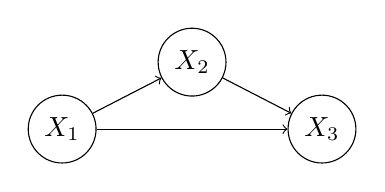
\begin{tikzpicture}
        \node (X1)  at (-1.65, 0) [circle, draw]{$X_1$};
        \node (X2) at (0, 0.85) [circle, draw]{$X_2$};
        \node (X3) at (1.65,0) [circle,draw]{$X_3$};
        % \node (Y)  at (1.75, 0) [circle, draw]{$\widehat{Y}$};
        \draw[->] (X1) to (X2) {};
        \draw[->] (X1) to (X3) {};
        % \draw[->] (X1) to (Y) {};
        \draw[->] (X2) to (X3) {};
        % \draw[->] (X2) to (Y) {};
    \end{tikzpicture}
\end{figure}
\end{minipage}
\begin{minipage}{.45\linewidth}
\begin{align*}
\mathcal{M} \, & 
\begin{cases}
    X_1 & \leftarrow U_1 \\
    X_2 & \leftarrow \alpha \cdot X_1  + U_2 \\
    X_3 & \leftarrow \beta_1 \cdot X_1 + \beta_2 \cdot X_2 + U_3
\end{cases}
\end{align*}
\end{minipage}
%

\medskip

\noindent
where $U_1, U_2, U_3$ represent the latent variables, $X_1, X_2, X_3$ the observed variables, and $\alpha, \beta_1, \beta_2$ the coefficient for the causal effect of, respectively, $X_1 \rightarrow X_2$,  $X_1 \rightarrow X_3$, and $X_2 \rightarrow X_3$. 
Suppose we want to generate the counterfactual for $X_3$, i.e., $X_3^{CF}$, had $X_1$ been equal to $x_1$. 
In the \textbf{abduction step}, we estimate $U_1$, $U_2$, and $U_3$ given the evidence, or what is observed, under the specified structural equations:
%
\begin{align*}
    \hat{U}_1 & = X_1 \\
    \hat{U}_2 & = X_2 - \alpha \cdot X_1 \\
    \hat{U}_3 & = X_3 - \beta_1 \cdot X_1 + \beta_2 \cdot X_2
\end{align*}
%
We generalize this step for \eqref{eq:SCM} as $U_j = X_j - f_j(X_{pa(j)})$ $\forall X_j \in X$. 
This step is an individual-level statement on the residual variation under SCM $\mathcal{M}$. 
It accounts for all that our assignment functions $f_j$, which are at the population level, cannot explain:~i.e., the \textit{error terms}. 
In the \textbf{action step}, we intervene $X_1$ and set all of its instances equal to $x_1$ via $do(X_1:=x_1)$ and obtain the intervened DAG $\mathcal{G}'$ and SCM $\mathcal{M}'$:

%
\begin{minipage}{.45\linewidth}
\begin{figure}[H]
\centering
    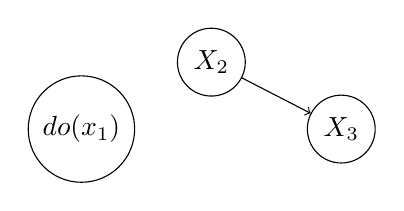
\begin{tikzpicture}
        \node (X1)  at (-1.65, 0) [circle, draw]{$do(x_1)$};
        \node (X2) at (0, 0.85) [circle, draw]{$X_2$};
        \node (X3) at (1.65,0) [circle,draw]{$X_3$};
        % \node (Y)  at (1.75, 0) [circle, draw]{$\widehat{Y}$};
        % \draw[->] (X1) to (X2) {};
        % \draw[->] (X1) to (X3) {};
        % \draw[->] (X1) to (Y) {};
        \draw[->] (X2) to (X3) {};
        % \draw[->] (X2) to (Y) {};
    \end{tikzpicture}
\end{figure}
\end{minipage}
\begin{minipage}{.45\linewidth}
\begin{align*}
\mathcal{M}' \, & 
\begin{cases}
    X_1 & = x_1 \\
    X_2 & \leftarrow \alpha \cdot x_1  + U_2 \\
    X_3 & \leftarrow \beta_1 \cdot x_1 + \beta_2 \cdot X_2 + U_3
\end{cases}
\end{align*}
\end{minipage}
%
\medskip

\noindent
where no edges come out from $X_1$ as it has been fixed to $x_1$. 
Finally, in the \textbf{prediction step}, we combine these two steps to calculate $X_3^{CF}$ under $\hat{U}$ and $\mathcal{M}'$:
%
\begin{align*}
    % X_1 &:= U_1 \\
    X_3^{CF} & \leftarrow \beta_1 \cdot x_1 + \beta_2 \cdot X_2 + \hat{U}_3 \\
             & \leftarrow \beta_1 \cdot x_1 + \beta_2 \cdot (\alpha \cdot x_1 + \hat{U}_2) + \hat{U}_3
\end{align*}
%
which is done for all instances in $X_3$. 
% This is what is done at a larger scale, for example, in \cite{Karimi2021_AlgoRecourse} and \cite{Pearl2016_CausalInference}, and also in this paper. 
The same three steps apply to $X_2$ and $X_1$.

We view the above approach as \textit{frequentist}, in particular, with regard to the abduction step.
% \footnote{This is not a formal distinction, but based on talks with other researchers. Such a distinction, to the best of our knowledge, remains an open question.} 
A more \textit{Bayesian} approach is what is done by \textcite{Kusner2017CF} in which they use a Monte Carlo Markov Chain (MCMC) to draw $\hat{U}$ by updating its prior distribution with the evidence $X$. 
In Section~\ref{sec:Experiments}, we used both approaches and found no difference in the results. 
In this work, we only present the results for the ``frequentist approach'' as it is less computationally expensive than running a MCMC. 

\section{Supplementary Material}
\label{Appendix.Supplements}

In this section, we present the supplementary material.

\subsection{Algorithms}

%
\begin{algorithm2e}[t]
\small %\scriptsize
    \caption{CST w/o $(\mathcal{D}, k, \tau, d)$}
    \label{alg:run_cfST}
	\SetKwInOut{Input}{Input}
	\SetKwInOut{Output}{Output}
	\Input{$\mathcal{D}$ - dataset, $k$ - neighborhood size, $\tau$ accepted deviation, $d$ distance function}
	\Output{$\mathcal{R}$ - set of pairs $(c, \Delta)$ of protected instance indexes and their $\Delta > \tau$}
	\BlankLine
	$\mathcal{D}_c=\{(x_i, a_i, \widehat{y}_i) \in \mathcal{D}: a_i=1\}$; \hfill\texttt{\scriptsize// control search space}\\
    $\mathcal{D}_t=\{(x_i, a_i, \widehat{y}_i) \in \mathcal{D}: a_i=0\}$\hfill\texttt{\scriptsize// test search space}\\
    $\mathcal{R} = \emptyset$\\
	\For{$(x_c, a_c, \widehat{y}_c) \in \mathcal{D}_c$}{
    $\text{\textit{k-ctr}} =
    \{ (x_i, a_i, \widehat{y}_i) \in \mathcal{D}_c: rank_{d}( x_c, x_i) \leq k \}$\hfill\texttt{\scriptsize// control group}\\
    $\text{\textit{k-tst}} = \{ (x_i, a_i, \widehat{y}_i) \in \mathcal{D}_t: rank_{d}( x^{CF}_c, x_i) \leq k \}$\hfill\texttt{\scriptsize// test group}\\
    $p_c = |\{ (x_i, a_i, \widehat{y}_i) \in \text{\textit{k-ctr}}: \hat{y}_i = 0 \}|/{k}$\hfill\texttt{\scriptsize// fraction of negative decisions for control}\\
    $p_t = |\{ (x_i, a_i, \widehat{y}_i) \in \text{\textit{k-tst}}: \hat{y}_i = 0 \}|/{k}$\hfill\texttt{\scriptsize// fraction of negative decisions for test}\\
    $\Delta = p_c - p_t$\hfill\texttt{\scriptsize// delta}\\
    \If{$\Delta > \tau$}{
    $\mathcal{R} = \mathcal{R} \cup \{(c, \Delta)\}$\hfill\texttt{\scriptsize// add pair to the result}\\
    }
	}
    \Return{$\mathcal{R}$}
\end{algorithm2e}
%

Algorithm~\ref{alg:run_cfST} reports the pseudo-code of the k-NN CST w/o algorithm. The pseudo-code is self-explanatory. 
After selecting the control and test search space (lines 1--2) as stated in Definition~\ref{def:SearchSpaces}, the algorithm iterates over the protected instances. For each of such instances, i.e., the complainant $c$, it builds (lines 5--6) the control and test groups as the $k$-nearest neighborhood instances relative to the distance $d$ for $x_c$ and for its counterfactual~$x^{CF}_c$ respectively, as stated in \eqref{eq:kctr} and \eqref{eq:ktst}. Then, the fractions $p_c$ and $p_t$ of negative decisions for the two groups are computed (lines 7--8) as stated in \eqref{eq:p1_and_p2}, as well as their difference $\Delta$ (line 9). If such a $\Delta$ is larger than the accepted deviation $\tau$, then the complainant $c$ and its $\Delta$ are added (lines 10--11) to the result $\mathcal{R}$.
%
The pseudo-code of k-NN CST w/ is a simple variant of Algorithm~\ref{alg:run_cfST}, which adds the search centers $x_c$ and $x^{CF}_c$ into the control and test groups, respectively, and divides by $k+1$ instead of $k$ at lines 7--8.

\subsection{Positive Discrimination}

Based on the discussion in Section~\ref{sec:CST_Disc}, we revisit Definitions \ref{def:IndDisc} and \ref{def:CIs} for testing individual positive discrimination under the k-NN CST. We still consider $\Delta p$ \eqref{eq:delta} and the converse of the one-sided CI $\eqref{eq:CIs}$. 

%
\begin{definition}[Positive Individual Discrimination]
\label{def:PostIndDisc}
    There is (potential) positive individual discrimination in favor of the complainant $c$ if $\Delta p < \tau$, meaning the negative decision outcomes rate for the control group is smaller than for the test group given some accepted deviation $\tau \in  [-1, 1]$.
\end{definition}
%

%
\begin{definition}[Confidence on the Positive Individual Discrimination Claim]
\label{def:PostCIs}
    A detected (potential) positive discrimination claim for the complainant $c$ by Definition~\ref{def:IndDisc}
    % by $\Delta p$ \eqref{eq:delta}  
    is statistically significant with significance level $\alpha$ if the CI $(- \infty, \Delta p + w_\alpha]$ excludes $\tau$.
\end{definition}
%

The concept of positive discrimination also applies to the case of multidimensional discrimination in Section~\ref{sec:CST.Multi}.
In that case, we would re-visit Definitions \ref{def:MultipleDisc} and \ref{def:IntersectionaleDisc} by looking at the opposite effect for $\Delta p$ across the protected attributes, be it each one of them or their intersection. 
We do not proceed with redefining these two definitions as we do not showcase them.
Again, especially for multidimensional discrimination, our focus is on discrimination \textit{against} protected groups.
Further, it is unclear what the legal scholarship views as positive multidimensional discrimination: from \textcite{Crenshaw1989_DemarginalizingTheIntersection} to \textcite{Xenidis2020_TunningEULaw}, the focus has been always on traditional discrimination.

\section{Additional Experiments}
\label{Appendix.AddExperiments}

In this section, we present additional experiments relative to the setup of Section~\ref{sec:Experiments}.

\subsection{Single Positive Discrimination}

For the same setup as in Section~\ref{sec:Experiments.SetUp} and the same data (factual and counterfactual) as in Section~\ref{sec:Experiments.IllustrativeExample}, we test for positive discrimination using Definitions \ref{def:PostIndDisc} and \ref{def:PostCIs}.
Regarding counterfactual fairness (CF), we define as positive CF discrimination when the factual has a positive decision outcome, $\hat{y}_c=1$ but its counterfactual a negative one, $\hat{y}_c^{CF}=0$.
Table~\ref{table:k-results_pos} summarizes the results for the protected attribute gender.

%
\begin{table}[t]
  \caption{Number (and \% females) of positive individual discrimination cases in Section~\ref{sec:Experiments.IllustrativeExample} based on gender. Marked by * are the statistically significant cases}
  \label{table:k-results_pos}
  \centering
  \begin{tabular}{clllll}
    \toprule
    Method & $k=15$ & $k=30$ & $k=50$ & $k=100$ & $k=250$\\
    \midrule
    CST w/o & 0 (0.0\%) & 0 (0.0\%) & 0 (0.0\%) & 0 (0.0\%)  & 0 (0.0\%) \\
     & 0* (0.0\%) & 0* (0.0\%) & 0* (0.0\%) & 0* (0.0\%)  & 0* (0.0\%) \\
     \midrule
    ST & 45 (2.6\%) & 50 (2.9\%) & 77 (4.5\%) & 118 (6.9\%) & 159 (9.3\%) \\
    & 41* (2.4\%) & 48* (2.8\%) & 55* (3.2\%) & 93* (5.4\%) & 120 (7.0\%) \\
    \midrule
    CST w/ & 0 (0.0\%) & 0 (0.0\%) & 0 (0.0\%) & 0 (0.0\%)  & 0 (0.0\%)\\
    & 0* (0.0\%) & 0* (0.0\%) & 0* (0.0\%) & 0* (0.0\%)  & 0* (0.0\%) \\
    \midrule
    CF & 0 (0.0\%) & 0 (0.0\%) & 0 (0.0\%) & 0 (0.0\%)  & 0 (0.0\%) \\
    & 0* (0.0\%) & 0* (0.0\%) & 0* (0.0\%) & 0* (0.0\%)  & 0* (0.0\%) \\
    \bottomrule
  \end{tabular}
\end{table}
%

Unlike all other single discrimination testing results in Section~\ref{sec:Experiments}, Table~\ref{table:k-results_pos} shows a ST that detects more cases than CST and a CST and CF that detect no cases at all. 
Both patterns hold when considering statistical significance.
These results are to be expected given how we generated the synthetic data for the loan application scenario. 
As described in Figure~\ref{fig:KarimiV2}, we introduced a negative systematic bias against female applicants in $\mathcal{D}$. 
This would explain why all the methods based on counterfactual generation---CF, CST w/, and CST w/o---detect zero cases: the generated male counterfactuals in $\mathcal{D}^{CF}$ can only improve over their female factual complainants in $\mathcal{D}$.
Hence, $\Delta p < \tau$ is very unlikely to occur when using CST or CF.
In other words, in a setting in which the protected individuals are always negatively affected in a systematic way, we should not expect to detect positive discrimination under methods that operationalize fairness given the difference.
Such results, for the purpose of this work, support our choice to consider only traditional discrimination as it is the most prevalent and important kind of discrimination when we suspect a negative systematic bias against the complainants. 

% Notably, 
Table~\ref{table:k-results_pos} raises questions on what kind of comparison is better suited for testing positive discrimination. 
The fact that ST, which uses an idealized comparison by implementing the CP manipulation, detects discrimination cases in a known biased setting for female applicants puts further into question the role of standard methods like it.
Is the idealized comparison suitable for positive discrimination or does \textcite{Kohler2018CausalEddie}'s criticism also apply to this setting?
Based on these preliminary results, we would argue that the tension between \textit{ceteris paribus} and \textit{mutatis mutandis} manipulations applies also to testing positive discrimination.
The stark difference between ST and CST in Table~\ref{table:k-results_pos} reinforces our view as, essentially, once we account for fairness given the difference in a known biased setting, it is difficult to argue that such a thing as positive discrimination occurs at all. 
Perhaps this is why this kind of discrimination is not discussed as much by legal scholars looking at indirect discrimination.
We plan to revisit these results in future work.

\subsection{Single Discrimination Testing}

We re-run Section~\ref{sec:Experiments.IllustrativeExample} and \ref{sec:Experiments.Real} for $\tau=0.05$, keeping all other parameters equal.
The results align with the ones we present in the main body. 
We focus on individual discrimination for all cases, not distinguishing between statistically and non-statistically significant cases.

Table~\ref{table:k-results_tau005} shows the same pattern between the CST versions relative to ST and CF as in Table~\ref{table:k-results}.
It illustrates the robustness of our framework. 
Two points we want to raise regarding Table~\ref{table:k-results_tau005}. 
First, CF, as expected, detects the same number of cases as it always looks for the strict equality between the factual and counterfactual quantities.
Second, under $\tau=0.05$, CST w/ and CST w/o align in the number of cases for larger $k$ sizes. This shows how influential $\tau$ can be for detecting discrimination, but also shows that either CST version can tackle the discrimination problem.
%
Tables \ref{table:k-results_RACE_tau005} and \ref{table:k-results_GENDER_tau005} show similar results as in, which are the $\tau=0.05$ counterparts of Tables \ref{table:k-results_RACE} and \ref{table:k-results_GENDER}. 
The results are expected given the setup. 
For both experiments the number of cases drops under $\tau=0.05$ as we have increased the difficulty of proving the individual discrimination claims.

%
\begin{table}[H]
  \caption{Number and (\% w.r.t. females) of cases based on $A$ in Figure~\ref{fig:KarimiV2}.}
  \label{table:k-results_tau005}
  \centering
  \begin{tabular}{lcccc}
    \toprule
    Method & $k=15$ & $k=30$ & $k=50$ & $k=100$ \\
    \midrule
    CST w/o & 288 (16.8\%) & 307 (17.9\%) & 331 (19.3\%) & 360 (21.0\%)  \\
    ST & 55 (3.2\%) & 60 (3.5\%) & 75 (4.4\%) & 79 (4.6\%) \\
    CST w/ & 420 (24.5\%) & 309 (18.1\%) & 334 (19.5\%) & 363 (21.2\%)  \\
    CF &  376 (22\%) &  376 (22\%) &  376 (22\%) & 376 (22\%)  \\
    \bottomrule
  \end{tabular}
\end{table}
%

%
\begin{table}[H]
  \caption{Number (and \% w.r.t.~non-whites) of cases based on $R$ using Figure~\ref{fig:LawSchool}.}
  \label{table:k-results_RACE_tau005}
  \centering
  \begin{tabular}{lccccc}
    \toprule
    Method & $k=15$ & $k=30$ & $k=50$ & $k=100$ \\
    \midrule
    CST w/o & 256 (7.30\%) & 301 (8.59\%) & 323 (9.21\%) & 376 (10.72\%)  \\
    ST & 33 (0.94\%) & 48 (1.37\%) & 57 (1.63\%) & 46 (1.31\%) \\
    CST w/ & 286 (8.16\%) & 301 (8.59\%) & 323 (9.21\%) & 376 (10.72\%)  \\
    CF &  231 (6.59\%) &  231 (6.59\%) &  231 (6.59\%) & 231 (6.59\%)  \\
    \bottomrule
  \end{tabular}
\end{table}
%
%
\begin{table}[H]
  \caption{Number (and \% w.r.t.~females) of cases based on $G$ Figure~\ref{fig:LawSchool}.}
  \label{table:k-results_GENDER_tau005}
  \centering
  \begin{tabular}{lcccc}
    \toprule
    Method & $k=15$ & $k=30$ & $k=50$ & $k=100$ \\
    \midrule
    CST w/o & 78 (0.82\%) & 105 (1.10\%) & 224 (2.35\%) & 231 (2.42\%)  \\
    ST & 77 (0.81\%) & 92 (0.96\%) & 181 (1.90\%) & 185 (1.94\%) \\
    CST w/ & 99 (1.04\%) & 105 (1.10\%) & 224 (2.35\%) & 231 (2.42\%)  \\
    CF &  56 (0.59\%) &  56 (0.59\%) &  56 (0.59\%) & 56 (0.59\%)  \\
    \bottomrule
  \end{tabular}
\end{table}
%

%
% EOS
%



% We present the relevant algorithms for the k-NN CST implementation (Section~\ref{sec:CST.AnImplementation}). The algorithm~\ref{alg:run_cfST} performs CST while algorithm~\ref{alg:get_topk} returns the indices of the top-$k$ tuples with respect to the search centers based on the distance function $d$. Notice that the main difference in algorithm~\ref{alg:run_cfST} when creating the neighborhoods is that the search centers are drawn from the factual dataset for the control group $\mathcal{D}$ and the counterfactual dataset $\mathcal{D}^{CF}$ for the test group. Further, notice that we use the same $c$ (i.e., index) for both as these two data-frames have the same structure by construction. 

% \newcommand\mycommfont[1]{\scriptsize\ttfamily\scriptsize{#1}}
% \SetCommentSty{mycommfont}

% \IncMargin{1.5em}
% \begin{algorithm2e}[h!]
% \small %\scriptsize
%     \caption{run\_CST}
%     \label{alg:run_cfST}
% 	\SetKwInOut{Input}{Input}
% 	\SetKwInOut{Output}{Output}
% 	\Input{$\mathcal{D}$, $\mathcal{D}^{CF}$, $k$}
% 	\Output{$[p_c - p_t]$}
% 	\BlankLine
% 	    $prot\_condition \leftarrow \mathcal{D}[:, \; prot\_attribute] == prot\_value$\\
% 	    $\mathcal{D}_c \leftarrow \mathcal{D}[prot\_condition]$\tcp*[f]{get protected (control) search space}\\
% 	    $\mathcal{D}_t \leftarrow \mathcal{D}[\neg \; prot\_condition]$\tcp*[f]{get non-protected (test) search space}\\
% 	    $prot\_idx \leftarrow \mathcal{D}_c.index.to\_list(\;)$\tcp*{get idx for all complainants}
% 	    $diff\_list = [ \; ]$ \\
% 	    \For{$c, \; row \in prot\_idx$}{
%         $res\_1 \leftarrow get\_top\_k(\mathcal{D}\; \; \; \; \; [c, \; :], \mathcal{D}_c, k)$\tcp*{idx of the top-k tuples for control group} 
%         $res\_2 \leftarrow get\_top\_k(\mathcal{D}^{CF}[c, \; :], \mathcal{D}_t, k)$\tcp*{idx of the top-k tuples for test group} 
%         $p_c \leftarrow sum(\mathcal{D}[res_1, \; target\_attribute]==negative\_outcome) \; / \; len(res\_1)$ \\
%         $p_t \leftarrow sum(\mathcal{D}[res_2, \; target\_attribute]==negative\_outcome) \; / \; len(res\_2)$ \\
%         $diff\_list[c] \leftarrow p_c - p_t$}
%     % \BlankLine
%     \Return{$diff\_list$}
%     % };\\ 
% \end{algorithm2e}

% \IncMargin{1.5em}
% \begin{algorithm2e}[h!]
% \small %\scriptsize
%     \caption{get\_top\_k}
%     \label{alg:get_topk}
% 	\SetKwInOut{Input}{Input}
% 	\SetKwInOut{Output}{Output}
% 	\Input{$t$, $t\_set$, $k$}
% 	\Output{$[indices]$}
% 	\BlankLine
%     % $(idx, dist) \leftarrow k\_NN(t, t\_set, k)$\tcp*{run k-NN algorithm}
%      $(idx, dist) \leftarrow k\_NN(t, t\_set, k + 1)$\tcp*{run k-NN algorithm with $k+1$}
%     \If{without search centers} {
%         $remove(t, idx, dist)$\tcp*{remove the center t from idx}
% %        \State $(idx, dist) \leftarrow k\_NN(t, t\_set, k + 1)$\tcp*{run k-NN algorithm with $k+1$}
%     }%\Else{
% %        \State $(idx, dist) \leftarrow k\_NN(t, t\_set, k)$\tcp*{run k-NN algorithm}
% %        \State $remove\_t(idx, dist)$\tcp*{remove the center t from idx}
% %    }
%     $idx' \leftarrow sort(idx, dist)$\tcp*{sort idx by the distance}
% %    \BlankLine
%     \Return{$idx'$}
%     % };\\ 
% \end{algorithm2e}




%%
\vskip 0.2in
\printbibliography
% \bibliography{references}
% \bibliographystyle{theapa}

\end{document}

%
% EOF
%
